\chapter{Experimentos y Resultados}
\label{chapter:experimentos}

En este capítulo se describen los experimentos llevados a cabo tanto para la
generación de \textit{streams} sintéticos como para el entrenamiento y
clasificación de modelos de \acrshort{mll}. Para comenzar, se presentan y
caracterizan las colecciones de datos utilizadas en las pruebas, luego se
detalla el ambiente en el cual se ejecutaron los experimentos, incluyendo
información sobre el hardware y software empleado. Una vez hecho esto, se listan
los algoritmos seleccionados para las pruebas, junto con la bibliografía
emparentada y la configuración particular de cada uno de ellos, y las métricas
de evaluación adoptadas y con las cuales se comparan los modelos. Ya en la
sección~\ref{configuracion_experimental} se entra en detalle sobre la
configuración de cada experimento, incluyendo hiperparámetros del entrenamiento,
métodos de evaluación de las clasificaciones y los tipos de \textit{streams}
generados. Finalmente, en la sección~\ref{experimentos_resultados} se exponen y
analizan los resultados.

\section{Colecciones}

\begin{table}[htbp]
	\centering
	\begin{tabular}{llrrrrr}
	\toprule
	Nombre    & Dominio & N     & A    & L   & LC    & LD    \\
	\midrule
	20ng      & Texto   & 19300 & 1006 & 20  & 1,029 & 0,051 \\
	Enron     & Texto   & 1702  & 1001 & 53  & 3,378 & 0,064 \\
	Mediamill & Video   & 43907 & 120  & 101 & 4,376 & 0,043 \\
	\bottomrule
\end{tabular}

	\caption[Colecciones multi-etiquetas y sus características.]{Colecciones
		multi-etiquetas y sus características. N:\@ número de
		instancias; A:\@ número de atributos; L:\@ número de etiquetas; LC:\@ cardinalidad
		de etiquetas; LD:\@ densidad de etiquetas.}
	\label{tab:datasets}
\end{table}

Se seleccionan colecciones de datos multi-etiquetas del mundo real que han sido
aplicados previamente en la literatura para evaluar la capacidad predictiva de
los modelos de
clasificación~\cite{osojnik_multi-label_2017,read_scalable_2012,buyukcakir_novel_2018}.
La tabla~\ref{tab:datasets} enumera sus características principales, incluyendo
métricas que describen su grado de multi-etiquetado (ver
sección~\ref{mll_def_formal}). Una descripción detallada de cada una se lista a
continuación:

\begin{description}

	\item{20ng}\footnote{\url{https://www.uco.es/kdis/mllresources/}}: Es una
	      colección que consta de casi 20 mil publicaciones provenientes de grupos de
	      noticias y que abordan 20 tópicos diferentes~\cite{lang_newsweeder_1995}.
	      La colección es de texto y fue preprocesada para formar 1006 atributos
	      numéricos.

	\item{Enron}\footnote{\url{http://sourceforge.net/projects/mulan/files/datasets/enron.rar}}:
	      Es una colección de correos electrónicos seleccionados de entre los 500
	      mil generados por empleados de la compañía eléctrica \textit{Enron} y
	      filtrados durante una investigación por
	      corrupción~\cite{hutchison_enron_2004}. Su tamaño, que no supera los
	      2000 elementos, no es lo suficientemente grande para ser considerado un
	      flujo continuo voluminoso, pero sí cuenta con otras propiedades como la
	      inclusión de fechas y una evolución de los datos en el
	      tiempo~\cite{read_scalable_2012}. Las etiquetas se dividen en cuatro
	      grupos, según su género (acuerdos laborales, correos meramente
	      personales, etc.); según la información que incluyen, esto es, si el
	      correo contiene enlaces externos, adjuntos, reenvíos, etc.; según el
	      tono emocional que reflejan y según el tópico principal que abordan.

	\item{Mediamill}\footnote{\url{https://sourceforge.net/projects/mulan/files/datasets/mediamill.rar}}:
	      Es una colección generada a partir de 80 horas de video provenientes de
	      transmisiones de noticias durante noviembre de
	      2004~\cite{snoek_challenge_2006}. Se seleccionaron más de 43 mil
	      ejemplos y fue manualmente etiquetada con 101 conceptos, que pueden
	      visualizarse en la figura~\ref{fig:mediamill}.

\end{description}

\begin{figure}[htbp]
	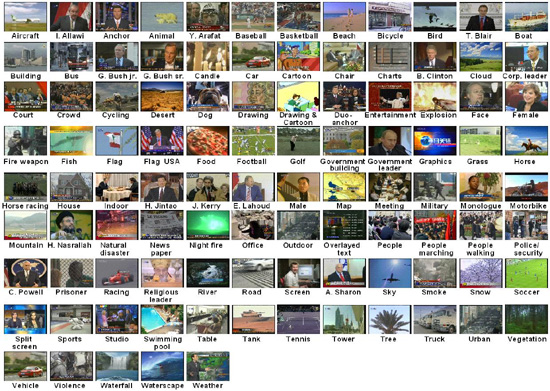
\includegraphics[width=.9\linewidth]{figures/mediamill.jpg}
	\centering
	\caption{Los 101 conceptos semánticos asociados a la colección
		Mediamill.}
	\label{fig:mediamill}
\end{figure}

Estas son solo tres de las colecciones usualmente abordadas en la literatura y
se han seleccionado con el objetivo de diversificar el análisis. Enron es una
colección de pocas instancias, pero muchas etiquetas, 20ng a la inversa, cuenta
con pocas etiquetas, pero muchas instancias; y Mediamill, finalmente, es la
colección con más instancias que hay disponible y cuenta también con un número
relativamente alto de etiquetas.

Durante la ejecución de experimentos, cada colección será convertida a un flujo
sintético. Además, se generará una versión sintética de cada una, siguiendo la
técnica descrita en la sección~\ref{generacion_flujos_sinteticos}.

\section{Software}

A continuación se describen las herramientas de software que fueron utilizadas
para la implementación y ejecución de los experimentos.

\begin{description}

	\item[scikit-multiflow]\footnote{\url{https://scikit-multiflow.github.io/}}
	      Es una librería disponible para el lenguaje de programación Python que
	      provee un \textit{framework} para implementar y comparar algoritmos de
	      aprendizaje automático en ambientes de flujos continuos de datos.
	      Incluye pero no se limita a problemas de clasificación
	      multi-etiquetas~\cite{montiel_scikit-multiflow_2018}.

	\item[\acrshort{moa}]\footnote{\url{https://moa.cms.waikato.ac.nz/}}
	      \acrfull{moa} es un \textit{framework} para realizar minería de datos
	      sobre flujos continuos de datos, implementada en Java y de código libre.
	      Incluye algoritmos de evaluación y de aprendizaje automático como
	      clasificadores, regresores, o de \textit{clustering}, pudiendo ser
	      aplicados a problemas de clasificación de etiqueta única o
	      multi-etiquetas.  También incluye herramientas para generar datos
	      sintéticos. Tanto \acrshort{moa} como scikit-multiflow facilitan la
	      reiteración de experimentos con distintas configuraciones, así como la
	      comparación de resultados y la extensión de
	      funcionalidad~\cite{bifet_moa_2010}.

	\item[scikit-learn]\footnote{\url{http://scikit-learn.org/stable/index.html}}
	      Es una librería del lenguaje de programación Python que brinda
	      herramientas para realizar evaluación, visualización y análisis de
	      resultados~\cite{pedregosa_scikit-learn_2018}.

	\item[Mulan]\footnote{\url{http://mulan.sourceforge.net/index.html}} Es una
	      librería del lenguaje Java especializada en aprendizaje por
	      multi-etiquetas. Mulan incluye una variedad de colecciones de datos
	      multi-etiquetas que han sido la fuente de otros trabajos de la
	      literatura~\cite{tsoumakas_mulan_2011}.

\end{description}

La herramienta \acrshort{moa} es usada para generar los flujos sintéticos y
provee del marco de trabajo en el cual se implementó el algoritmo de generación
descrito en~\ref{generacion_flujos_sinteticos}. Los algoritmos de clasificación
fueron implementados en Python y están disponibles bajo la librería
\textit{scikit-multiflow}. La solución de ensamble \acrshort{efmp} también fue
implementada en esta librería. \textit{Scikit-learn}, por su parte, provee la
implementación de las métricas basadas en etiquetas, y las colecciones de datos
fueron extraídas de Mulan.

\section{Hardware}

Se ha recibido apoyo del \acrfull{cidetic}, el cual ha proveído de equipos de
altas prestaciones que han proporcionado la capacidad de cómputo necesaria para
llevar a cabo este proyecto. El equipamiento facilitado cuenta con dos nodos de
12 núcleos cada uno, la CPU es un Intel Xeon X5675 de 3.07 GHz de velocidad de
procesamiento, 12 MB de memoria caché y 6 núcleos. El espacio de almacenamiento
disponible es de 1 TB y la memoria RAM es de 142 GB\@. \todo{Chequear estos datos}

El Sistema Operativo instalado es Ubuntu 18.04 LTS y cuenta con la versión 3.6.9
de Python, el instalador de paquetes Pip en su versión 20.3.3 y Java 1.8.

\section{Algoritmos}
\label{experimentos_algoritmos}

Se realizan los experimentos usando algoritmos multi-etiquetas disponibles en la
librería scikit-multiflow junto con las implementaciones de ensambles
presentadas en este trabajo: \acrfull{efmp} y su variación \acrshort{efmp2}.
Entre los algoritmos del tipo de transformación del problema se seleccionan los
de \acrfull{br}, \acrfull{cc} y \acrfull{mlht}. Tanto \acrshort{br} como
\acrshort{cc} usan \textit{naive} bayes como modelo de clasificación base y
\acrshort{mlht} es ejecutado en su versión basada en \acrfull{lp}, siguiendo los
procedimientos de \citeauthor{read_scalable_2012}~\cite{read_scalable_2012}.

En lo que respecta a soluciones de ensamble, los modelos de \acrshort{efmp}
contarán ambos con tres clasificadores base, siendo estos los mencionados en el
párrafo anterior, es decir, \acrshort{cc}, \acrshort{br} y \acrshort{mlht}. La
comparación se hará contra el algoritmo \acrfull{dwm}, tal como ha sido definido
por sus autores~\cite{kolter_dynamic_2007} pero adaptado a ambientes de
multi-etiquetas (ver sección~\ref{tecnica_algoritmo_ensamble}), y se suman al
análisis los algoritmos de \acrfull{ebr} y \acrfull{ecc}, tal como fueron
definidos por \citeauthor{oza_online_2005}~\cite{oza_online_2005} y también han
sido extendidos para soportar problemas de
\acrshort{mll}~\cite{read_classifier_2011}. Los tres algoritmos de ensamble
extraídos de la literatura son configurados con diez clasificadores base de
\textit{naive} bayes, para imitar los experimentos conducidos por otros autores
de la literatura~\cite{osojnik_multi-label_2017, read_scalable_2012,
	buyukcakir_novel_2018}.

La tabla~\ref{tab:algoritmos} es un resumen de los algoritmos seleccionados
junto con los clasificadores base configurados, la referencia bibliográfica y la
clave que será usada en las tablas de resultados.

\begin{table}[htbp]
	\centering
	\begin{adjustbox}{max width=\textwidth}
		\begin{tabular}{lllll}
	\toprule
	Clave                                          & Algoritmo                             & Clasificadores base  & Referencia & \\
	\midrule
	\acrshort{br}                                  & \acrlong{br}                          & \textit{naive} bayes
	                                               & \textcite{tsoumakas_multi-label_2007} &                                     \\
	\acrshort{cc}                                  & \acrlong{cc}                          & \textit{naive} bayes &
	\textcite{read_classifier_2011}                &                                                                             \\
	\acrshort{mlht}                                & \acrlong{mlht}                        & \acrfull{ht}         &
	\textcite{read_scalable_2012}                  &                                                                             \\
	\acrshort{efmp}                                & \acrlong{efmp}                        &
	\acrshort{br}, \acrshort{cc} y \acrshort{mlht} &
	Sección \ref{tecnica_algoritmo_ensamble}       &                                                                             \\
	\acrshort{efmp2}                               & \acrlong{efmp2}                       &
	\acrshort{br}, \acrshort{cc} y \acrshort{mlht} &
	Sección \ref{tecnica_algoritmo_ensamble}       &                                                                             \\
	\acrshort{dwm}                                 & \acrlong{dwm}                         &
	\textit{naive} bayes (10 copias)               &
	\textcite{kolter_dynamic_2007}                 &                                                                             \\
	\acrshort{ebr}                                 & \acrlong{ebr}
	                                               & \textit{naive} bayes (10
	copias)                                        &
	\textcite{read_classifier_2011}                &                                                                             \\
	\acrshort{ecc}                                 & \acrlong{ecc}
	                                               & \textit{naive} bayes (10
	copias)                                        &
	\textcite{read_classifier_2011}                &                                                                             \\
	\bottomrule
\end{tabular}

	\end{adjustbox}
	\caption{Métodos de clasificación multi-etiquetas seleccionados para ambientes
		de flujos continuos de datos.}
	\label{tab:algoritmos}
\end{table}

\section{Métricas de Evaluación}

En la evaluación de algoritmos de clasificación se usan el conjunto de métricas
que han sido utilizadas en otros trabajos de la literatura, tanto en escenarios
de
flujos~\cite{sousa_multi-label_2018,zheng_survey_2020,osojnik_multi-label_2017}
como en
\textit{batch}~\cite{madjarov_extensive_2012,zhang_multi-label_2010,gibaja_tutorial_2015}
y fueron descritas en la sección~\ref{mll_evaluacion}.  Estas son:

\begin{description}

	\item[Métricas Basadas en Ejemplos]: \textit{Hamming score}, \textit{hamming
		      loss}, \textit{exact-match} (exactitud del subconjunto),
	      \textit{accuracy} (o exactitud, o \textit{jaccard index}), precisión,
	      \textit{recall} (o exhaustividad) y \textit{f1}.

	\item[Métricas Basadas en Etiquetas]: \textit{Accuracy} (micro), precisión
	      (micro), \textit{recall} (micro), \textit{f1} (micro),
	      \textit{accuracy} (macro), precisión (macro), \textit{recall} (macro)
	      y \textit{f1} (macro).

	\item[Métricas de Eficiencia]: Velocidad y tamaño del modelo.

\end{description}

La medición de velocidad comienza en el momento que inicia la predicción y
entrenamiento del modelo por primera vez y finaliza cuando el clasificador
termina de procesar la última instancia de la colección. Por lo tanto, quedan
afuera las etapas de evaluación, carga de la colección en memoria, generación
del flujo y configuración del entrenamiento. El consumo de memoria también es
monitoreado durante la ejecución del entrenamiento y predicción y toma en cuenta
la estructura completa del modelo y todos sus componentes, incluyendo pesos e
hiperparámetros propios y de sus clasificadores base.

Los flujos sintéticos son analizados teniendo en cuenta los fenómenos propios de
colecciones del mundo real. A ese fin se estudia el sesgo de etiquetas, la
relación entre etiquetas, la distribución de etiquetas y el espacio de atributos
(ver sección~\ref{mll_fenomenos}).

\section{Configuración Experimental}
\label{configuracion_experimental}

En lo que respecta a modelos de aprendizaje automático, los experimentos fueron
desarrollados en el lenguaje Python usando la librería
\textit{scikit-multiflow}. Los algoritmos de transformación del problema se
aplican tal como han sido implementados en la librería con la salvedad del
\acrshort{mlht}, al que debió introducirle una modificación para manipular la
predicción, se usaba un arreglo disperso para representar las etiquetas
activadas, lo cual producía un desbordamiento de memoria en el entrenamiento de
colecciones grandes como la de Mediamill. Se lo suplantó por una estructura de
representación densa. En cuanto a los modelos de ensambles, se adaptaron las
implementaciones existentes de \acrshort{ebr}, \acrshort{ecc} y \acrshort{dwm}
para soportar múltiples etiquetas y para ello se debió modificar la etapa de
combinación de votos para hacer frente a la nueva dimensionalidad de los datos.
Por lo demás, la configuración de los algoritmos es la definida en la
sección~\ref{experimentos_algoritmos}.

Para la etapa de evaluación se aplica la técnica de evaluación secuencial
predictiva (\textit{prequential}) con ventanas deslizantes, tal como se
recomienda para ambientes de flujos continuos~\cite{gama_evaluating_2013}. Ante
cada ejemplo o ventana de ejemplos arribada el modelo primero realiza la
predicción y luego el entrenamiento. Finalmente, las métricas de evaluación son
calculadas una vez procesados todos los ejemplos de la colección y a partir de
todas las predicciones producidas.  Notar que a partir de esta técnica el modelo
predice y entrena todas las instancias, y no solo un subconjunto de ellas como
sucede con la estrategia de \textit{holdout}. La ventana deslizante se configura
en $w = \frac{N}{20}$, es decir, se divide el número total de instancias del
flujo en 20 ventanas, siguiendo las directivas de \textcite{read_scalable_2012}.
Los resultados de la evaluación son agrupados según los tipos de métrica usados,
para facilitar el análisis.

Por otro lado, los flujos de datos sintéticos fueron generados a partir de las
colecciones 20ng, Enron y Mediamill. Por cada uno de ellos se generan tres
\textit{streams} sintéticos:

\begin{description}

	\item[MOA]: Es un \textit{stream} generado usando el método de los autores
	      de referencia~\cite{read_generating_2009}. El número de instancias es el
	      mismo de la colección original y el generador de atributos es
	      \acrfull{rbf} (ver sección~\ref{stream_syn}).

	\item[JC]: Es un \textit{stream} generado usando el método presentado en la
	      sección~\ref{generacion_flujos_sinteticos}. El número de instancias es
	      el mismo de la colección original y el generador de atributos es
	      \acrfull{rbf}.

	\item[JC\_BIG]: Es un \textit{stream} similar a JC, pero cuenta con un mayor
	      número de instancias. La idea es poder determinar si a mayor el tamaño
	      del \textit{stream} mayor es la similitud con la colección original.

\end{description}

Una vez generados estos flujos sintéticos se realizó un análisis para determinar
en qué grado se observan los fenómenos de la colección original en las
colecciones sintéticas. Estos fenómenos son el sesgo de etiquetas, la
distribución de etiquetas, la relación entre etiquetas y el espacio de
atributos, y se capturaron siguiendo la metodología del trabajo de referencia,
esto es:

\begin{description}

	\item[Sesgo de etiquetas]: Para observar el sesgo de etiquetas se toma la
	      frecuencia de cada etiqueta y se traza un gráfico de línea para cada
	      \textit{stream}, de esta manera es posible visualizar cuánto se asemeja
	      el sesgo de los datos sintéticos al de los datos reales. Además, se
	      adjunta una tabla que lista las 5 combinaciones principales para cada
	      flujo continuo.

	\item[Distribución de etiquetas]: El objetivo de estudiar este fenómeno es
	      conocer de qué forma se compone la cardinalidad de etiquetas. Para ello
	      se traza un gráfico que exhibe la frecuencia escalada de cada tamaño de
	      etiquetas hallado en cada \textit{stream}. A su vez, se adjunta un
	      gráfico que aplica el \textit{mean absolute error} de cada flujo
	      continuo sintético sobre el de los datos originales, y así facilitar la
	      comparativa entre \textit{streams}. De manera complementaria,
	      \citeauthor{read_generating_2009} definen dos tipos de distribuciones de
	      etiquetas: tipo A y tipo B (ver sección~\ref{mll_fenomenos}). En la
	      sección de resultados se clasificarán los flujos sintéticos bajo esta
	      taxonomía.

	\item[Relación entre Etiquetas]: Este fenómeno se estudia observando la
	      aparición mutua de etiquetas. Para ello se genera un gráfico que pone de
	      manifiesto la matriz de co-ocurrencias de pares de etiquetas. El gráfico
	      es un mapa de colores de dos dimensiones donde la magnitud del color
	      está dada por la frecuencia en la que dos etiquetas han sido activadas
	      en conjunto.

	\item[Espacio de Atributos]: Se listan los atributos más frecuentes del
	      flujo original y de los flujos sintéticos.

\end{description}


\section{Resultados}
\label{experimentos_resultados}

A continuación se exhiben los resultados obtenidos de los experimentos. En
primer lugar, en la sección~\ref{experimentos_syn_streams} se estudian los
flujos continuos sintéticos generados y luego, ya en la
sección~\ref{experimentos_clasificaciones}, se analizan los resultados de las
evaluaciones.

\subsection{Flujos Continuos Sintéticos}
\label{experimentos_syn_streams}

El estudio de los \textit{streams} sintéticos generados se divide en tres
secciones, una para cada una de las colecciones. Cada sección incluye
una tabla con las características tanto del \textit{stream} basado en datos
reales como de los tres \textit{streams} sintéticos. Luego se analizan los
fenómenos propios de colecciones multi-etiquetadas y cómo estos se presentan en
los flujos sintéticos, con las particularidades observadas en cada caso.

\subsubsection{20ng}

La tabla~\ref{tab:syn_20ng_stats} muestra las características de la colección
original y de los \textit{streams}. Allí se observa que la cardinalidad de la
colección apenas sobrepasa la unidad, lo que significa que la mayoría de sus
instancias tienen una única etiqueta. Esta característica logra ser capturada de
manera aproximada por los \textit{streams} JC y JC\_BIG, pero no así por MOA que
asocia más de tres etiquetas por instancia.

\begin{table}[htbp]
	\centering
	\begin{adjustbox}{max width=\textwidth}
		\begin{tabular}{lrrrr}
	\toprule
	\multicolumn{5}{c}{20ng}             \\
	Nombre  & N     & L  & LC    & LD    \\
	\midrule
	20ng    & 19300 & 20 & 1,029 & 0,051 \\
	MOA     & 19300 & 20 & 3,397 & 0,170 \\
	JC      & 19300 & 20 & 1,067 & 0,053 \\
	JC\_BIG & 80000 & 20 & 1,062 & 0,053 \\
	\bottomrule
\end{tabular}

	\end{adjustbox}
	\caption[Características de los \textit{streams} sintéticos generados sobre
		la colección 20ng.]{Características de los \textit{streams} sintéticos
		generados sobre la colección 20ng.  N:\@ número de instancias; L:\@
		número de etiquetas; LC:\@ cardinalidad de etiquetas; LD:\@ densidad de
		etiquetas.}
	\label{tab:syn_20ng_stats}
\end{table}


La figura~\ref{fig:syn_20ng_label_skew} es una representación gráfica del sesgo
de etiquetas, y muestra que la colección original tiene alrededor de veinte
combinaciones con una frecuencia escalada cercana a la máxima y luego un
descenso brusco que culmina en la combinación 25, desde la cual se mantiene
cercana a la frecuencia escalada mínima. Esta tendencia es bien replicada en los
\textit{streams} JC, pero no en MOA, donde el descenso es más escalonado y no
alcanza la zona baja del eje y.

\begin{figure}[htbp]
	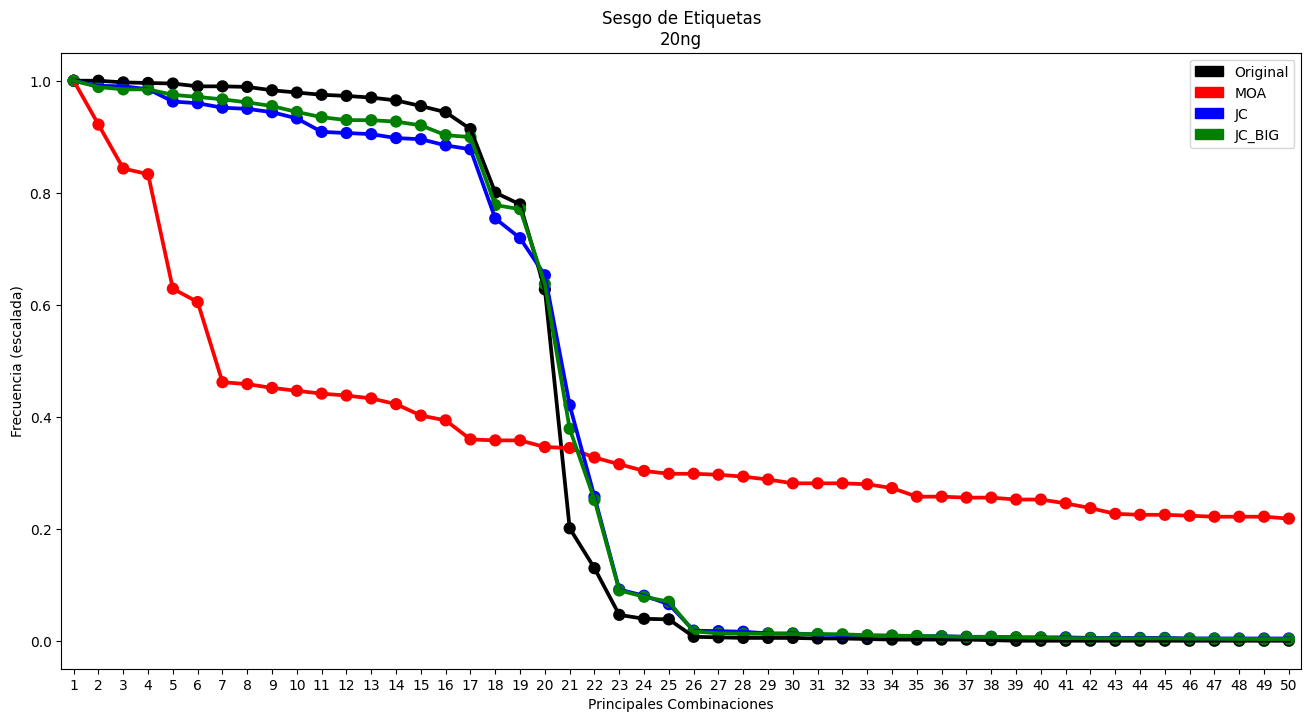
\includegraphics[width=\linewidth]{figures/experiments/syn/20ng/label_skew.png}
	\caption{Sesgo de etiquetas de los \textit{streams} generados sobre la colección
		20ng.}
	\label{fig:syn_20ng_label_skew}
\end{figure}

\begin{table}[htbp]
	\centering
	\begin{adjustbox}{max width=\textwidth}
		\begin{tabular}{lllll}
	\toprule
	\textit{Rank} & Original               & JC                     & JC\_BIG                & MOA                                                                                       \\
	\midrule
	1             & \{religion.christian\} & \{sci.crypt\}          & \{religion.christian\} & \{comp.os\_ms\_windows\_misc, religion.rmisc, misc\_forsale, comp.sys.ibm\_pc\_hardware\} \\[3pt]
	2             & \{rec.sport.hockey\}   & \{sci.med\}            & \{rec.motorcycles\}    & \{sci.space, rec.autos, rec.motorcycles, politics.guns, religion.atheism\}                \\[3pt]
	3             & \{sci.crypt\}          & \{religion.christian\} & \{rec.autos\}          & \{religion.rmisc, sci.space, misc\_forsale\}                                              \\[3pt]
	4             & \{rec.motorcycles\}    & \{sci.electronics\}    & \{sci.med\}            & \{sci.space, rec.motorcycles, politics.guns, religion.atheism\}                           \\[3pt]
	5             & \{rec.sport.baseball\} & \{rec.sport.hockey\}   & \{sci.electronics\}    & \{politics.pmisc, politics.mideast, rec.sport.hockey, sci.crypt\}                         \\
	\bottomrule
\end{tabular}


	\end{adjustbox}
	\caption{Sesgo de etiquetas: Principales combinaciones de los
		\textit{streams} generados sobre la colección 20ng.}
	\label{tab:syn_20ng_top_labels_combinations}
\end{table}

La tabla~\ref{tab:syn_20ng_top_labels_combinations} muestra las principales 5
combinaciones de etiquetas para cada \textit{stream}. Cabe destacar que todas
las combinaciones en la tabla para los \textit{streams} JC y JC\_BIG son de una
etiqueta cada una, tal como el original, pero además JC captura 3 de las 5
combinaciones principales del original: $\{religion.cristian\}$,
$\{rec.sport.hockey\}$ y $\{sci.crypt\}$.

\begin{figure}[htbp]
	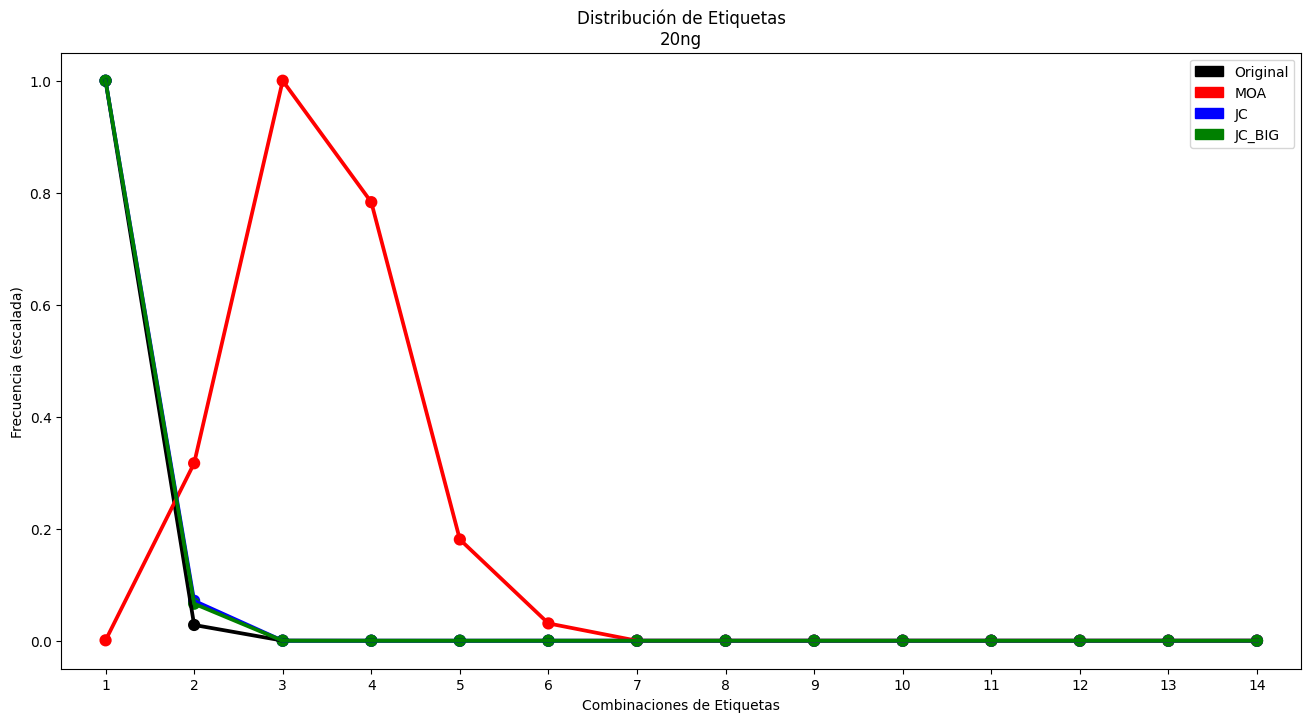
\includegraphics[width=\linewidth]{figures/experiments/syn/20ng/label_distribution.png}
	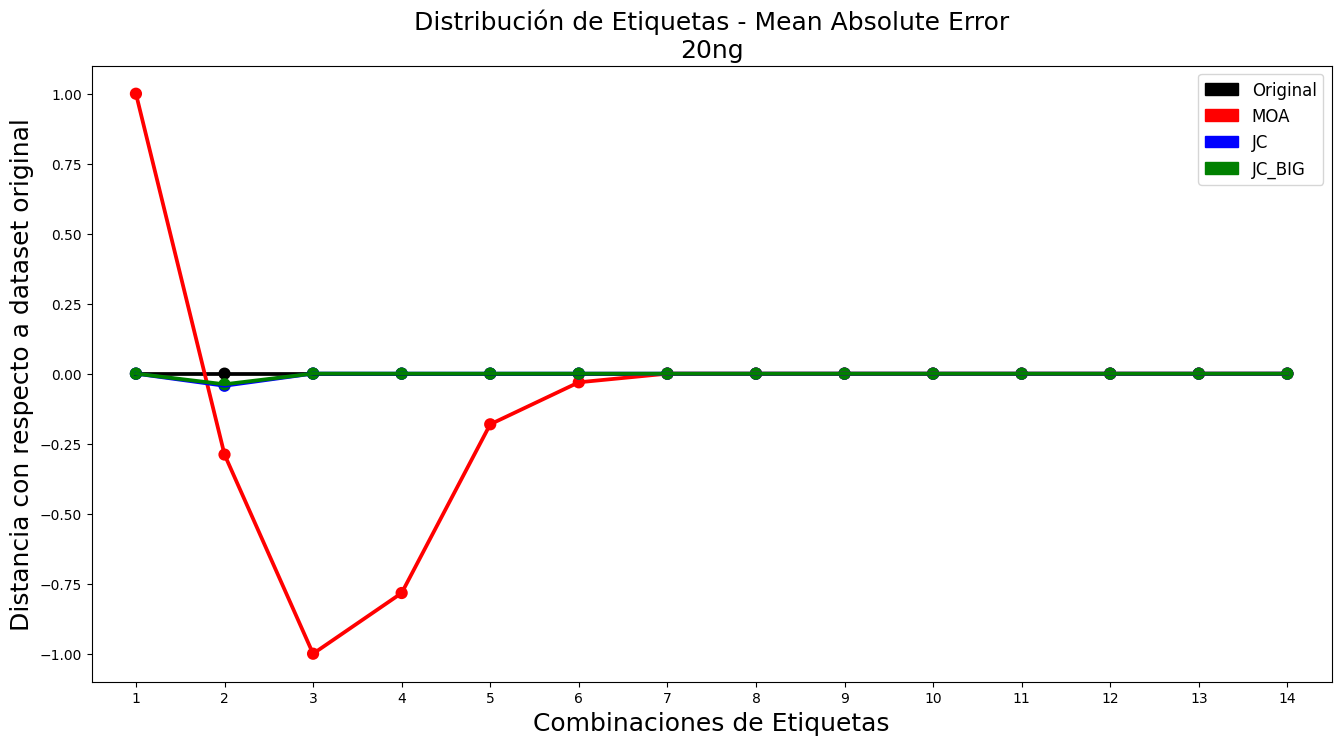
\includegraphics[width=\linewidth]{figures/experiments/syn/20ng/ld_mae.png}
	\caption[Distribución de etiquetas de los \textit{streams} generados sobre la colección
		20ng.]{Distribución de etiquetas de los \textit{streams} generados sobre la colección
		20ng. Arriba se encuentra el gráfico con las frecuencias escaladas y
		abajo el \textit{mean absolute error} entre cada \textit{stream} y la
		colección original.}
	\label{fig:syn_20ng_label_distribution}
\end{figure}

La figura~\ref{fig:syn_20ng_label_distribution} representa de manera gráfica la
distribución de las etiquetas. Allí se observa cómo los \textit{streams} aquí
presentados reproducen con eficacia la composición de la cardinalidad a lo largo
de los distintos tamaños de conjuntos de etiquetas. El gráfico de \textit{mean
	absolute error} ayuda a reforzar esta idea. En cuanto al tipo de distribución,
del cual se hace mención en el trabajo de referencia, los \textit{streams} JC y
JC\_BIG, tanto como el original, obedecen al tipo A, esto es, la mayoría de los
ejemplos tienen un conjunto de etiquetas de cardinalidad uno.

\begin{figure}[htbp]
	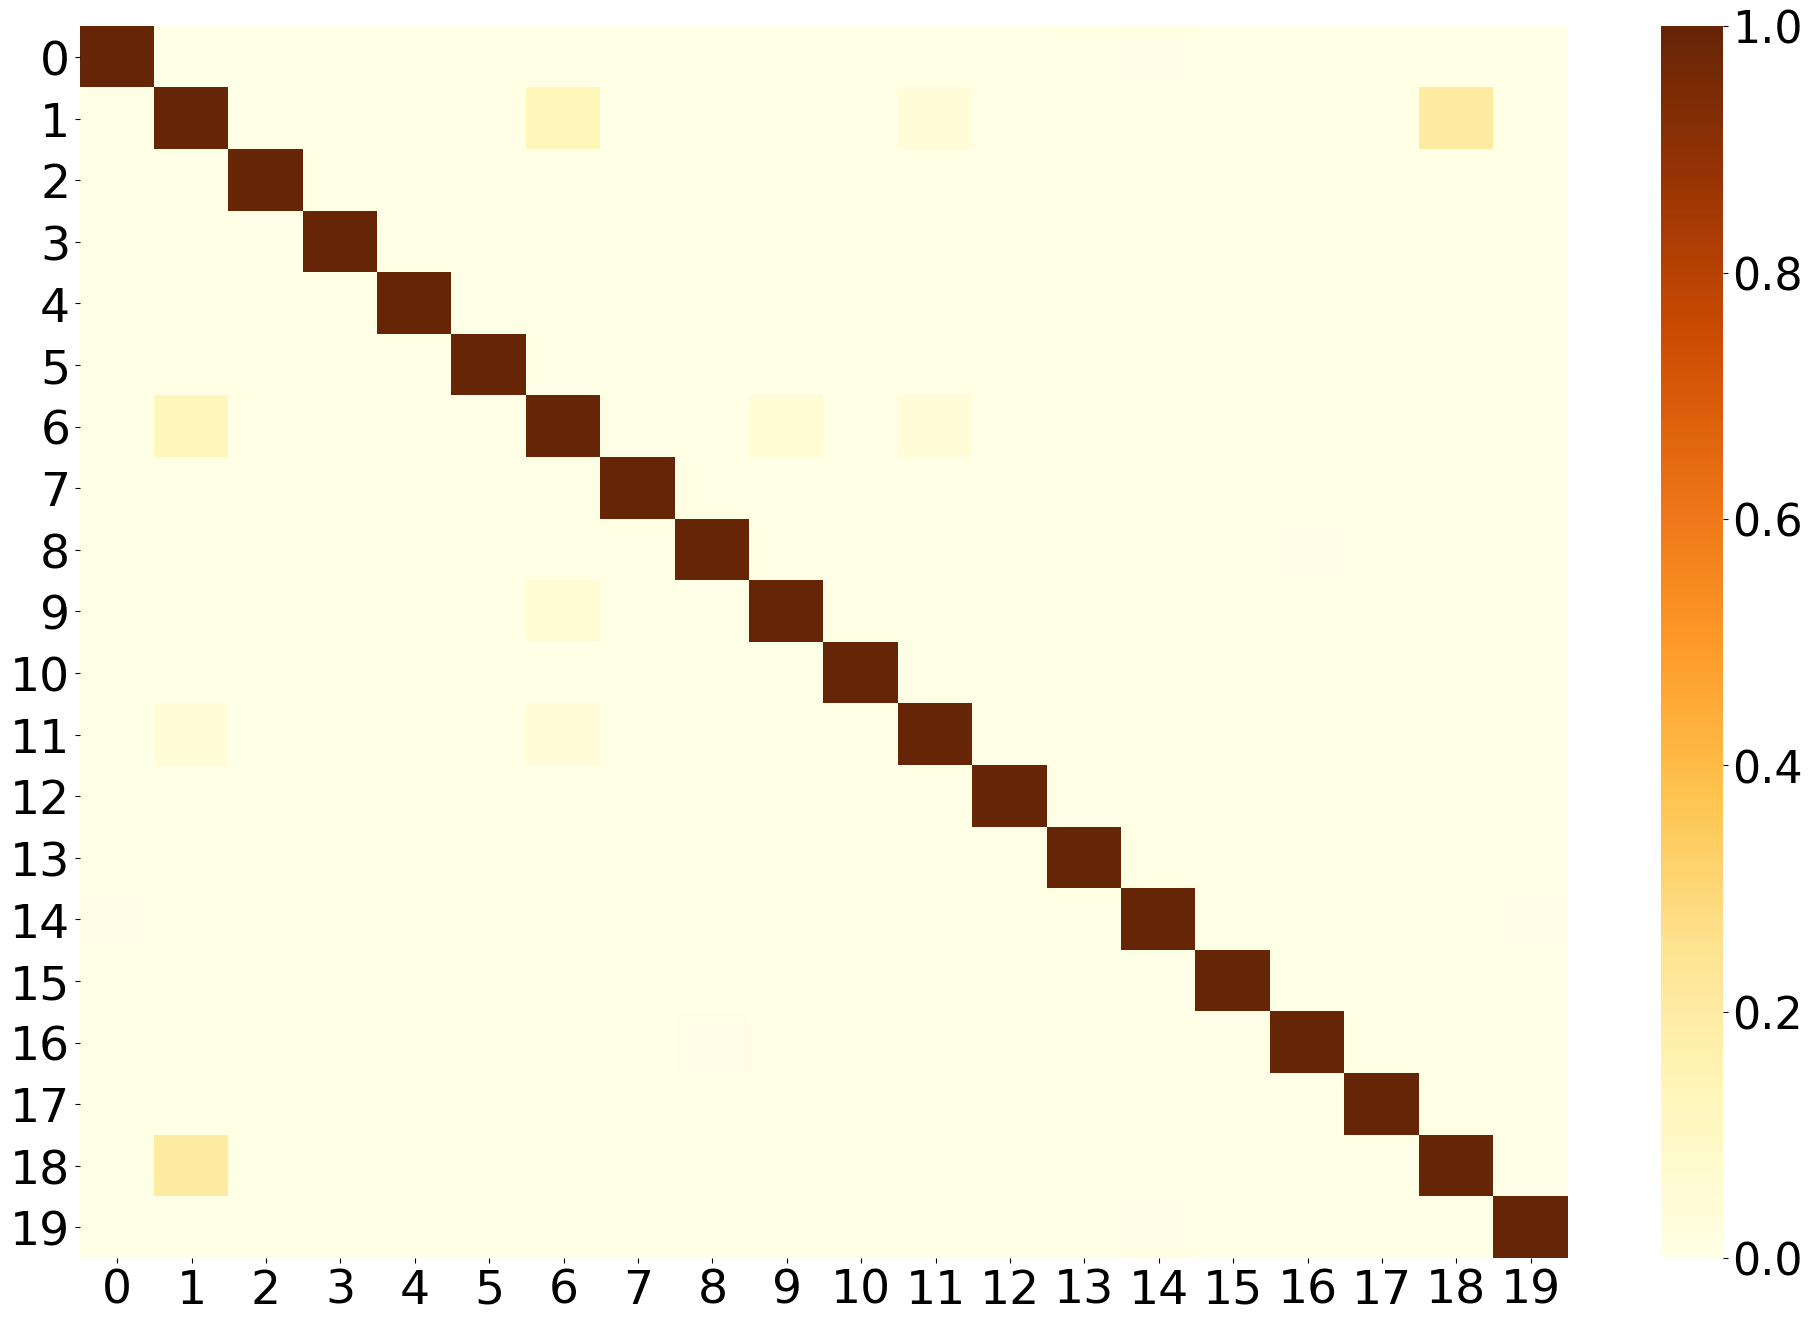
\includegraphics[width=\linewidth / 2]{figures/experiments/syn/20ng/20ng_relationship_graph.png}
	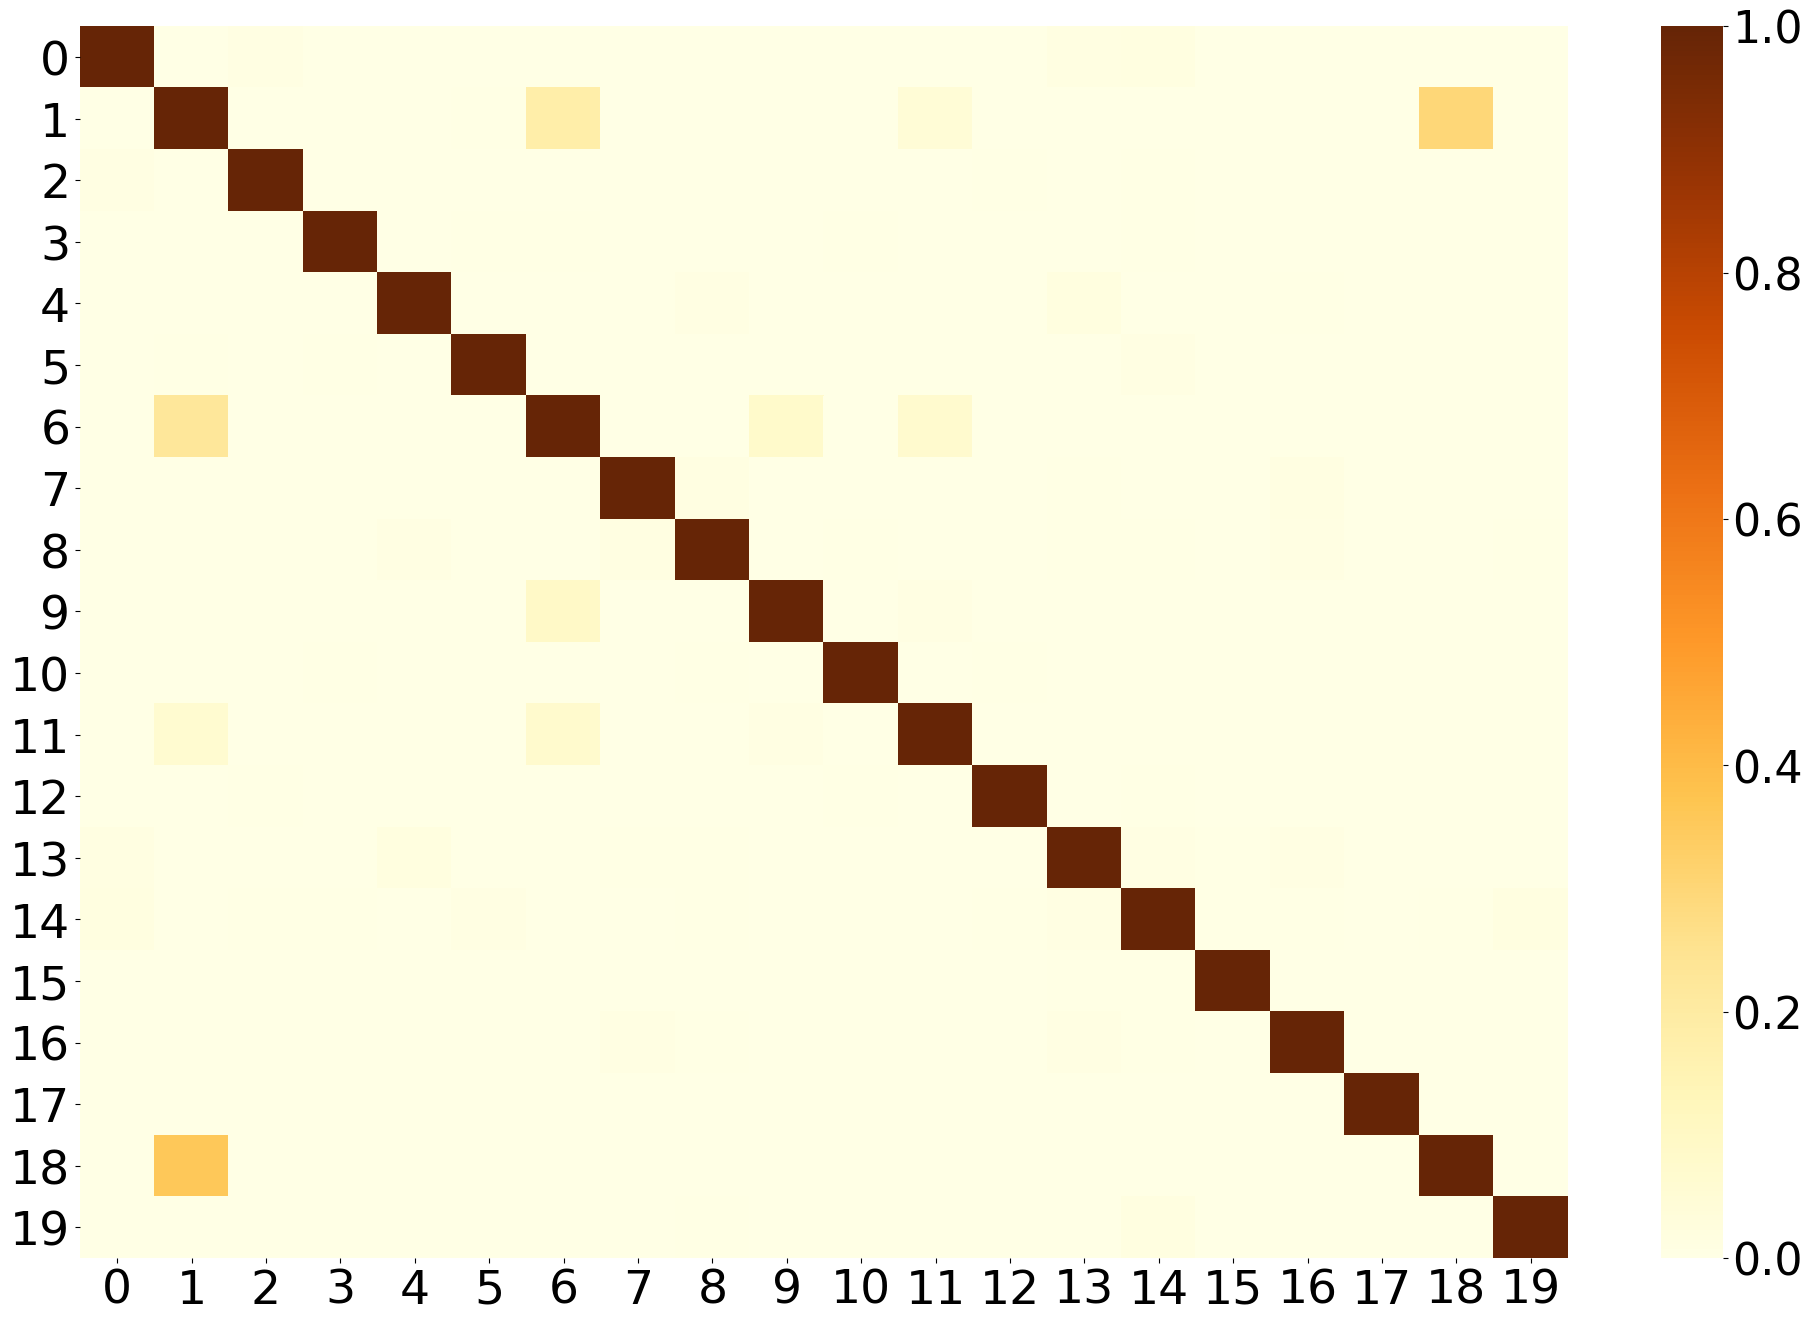
\includegraphics[width=\linewidth / 2]{figures/experiments/syn/20ng/JC_relationship_graph.png}
	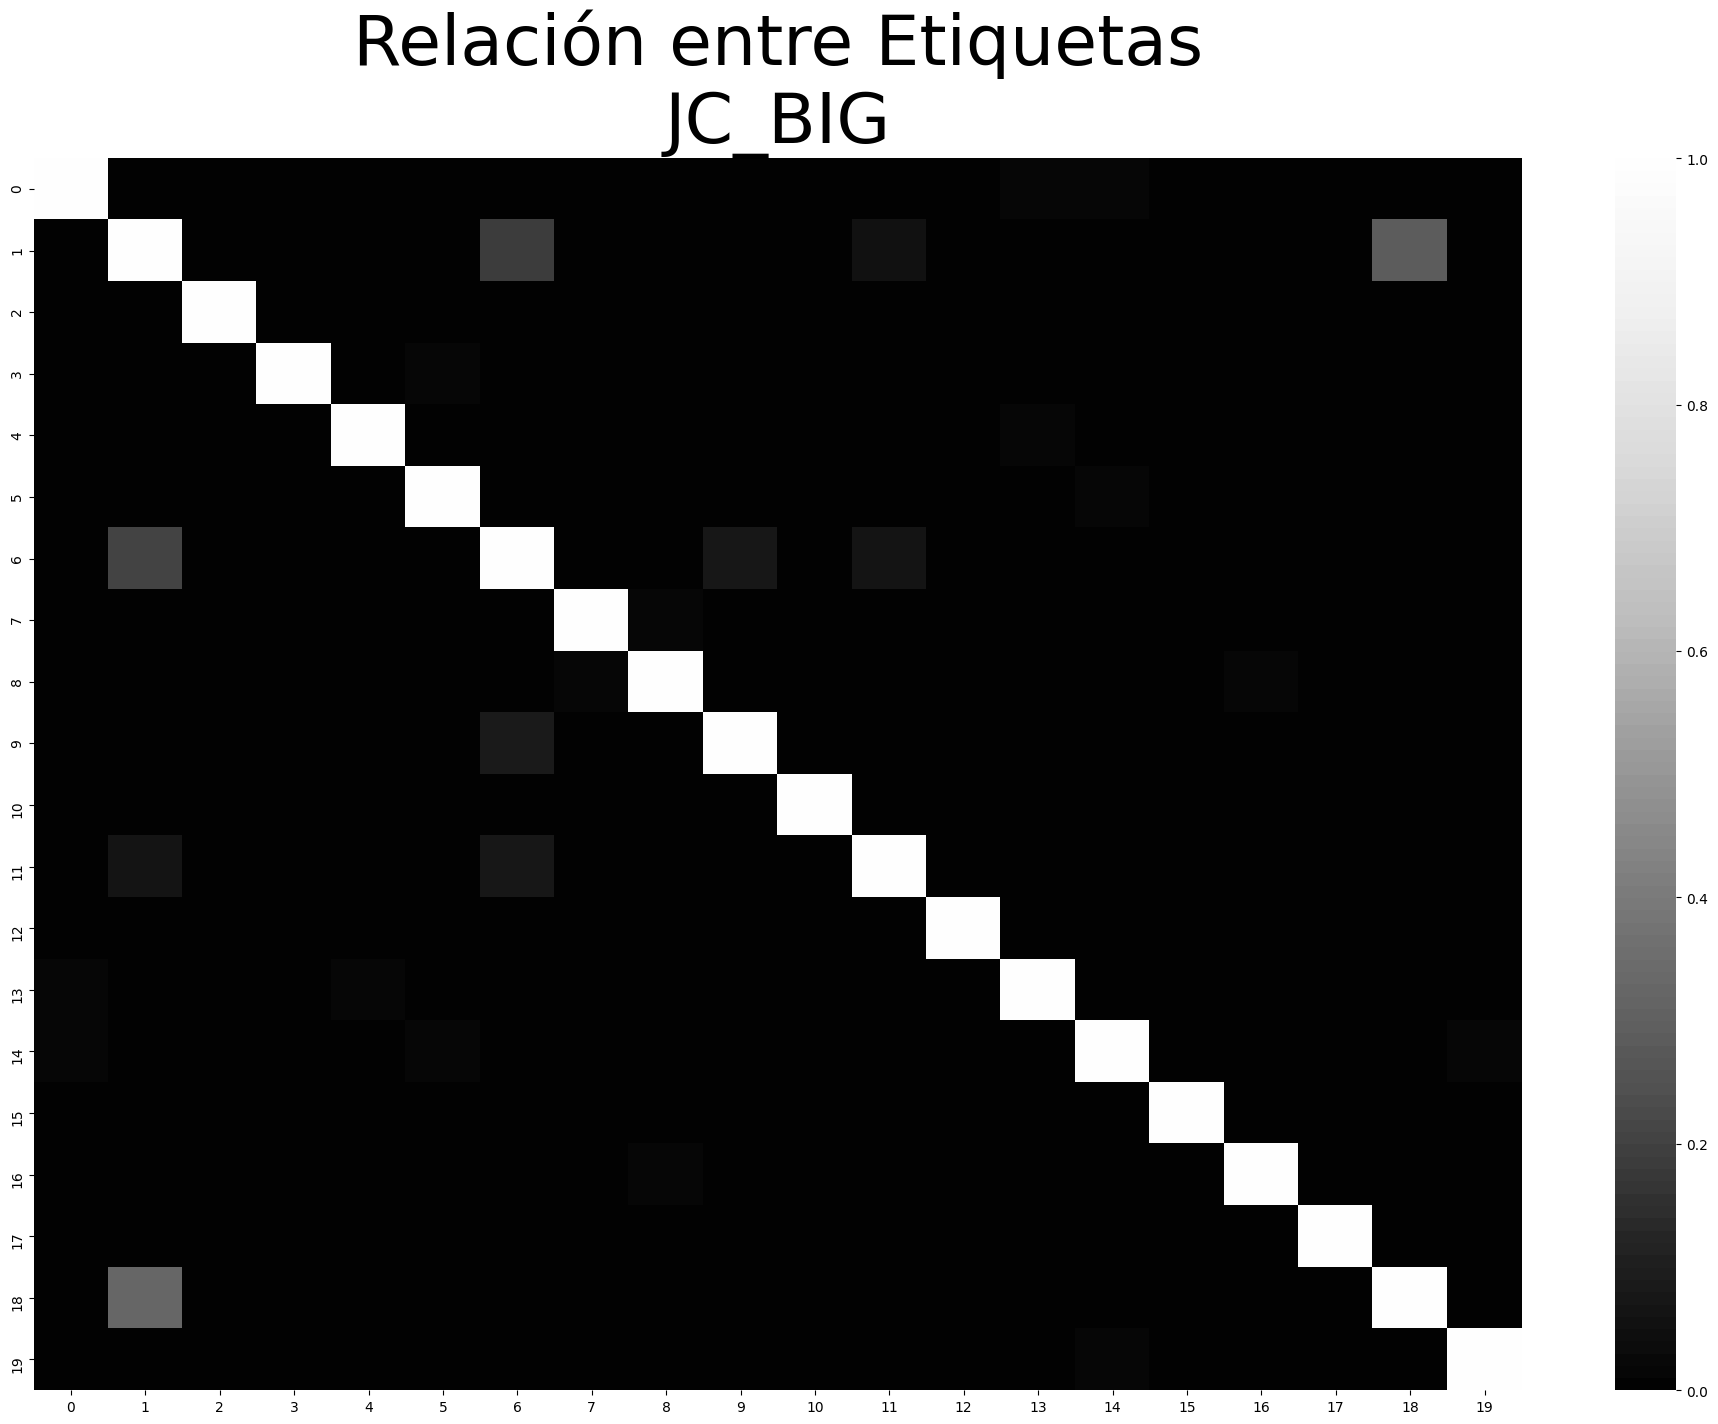
\includegraphics[width=\linewidth / 2]{figures/experiments/syn/20ng/JC_BIG_relationship_graph.png}
	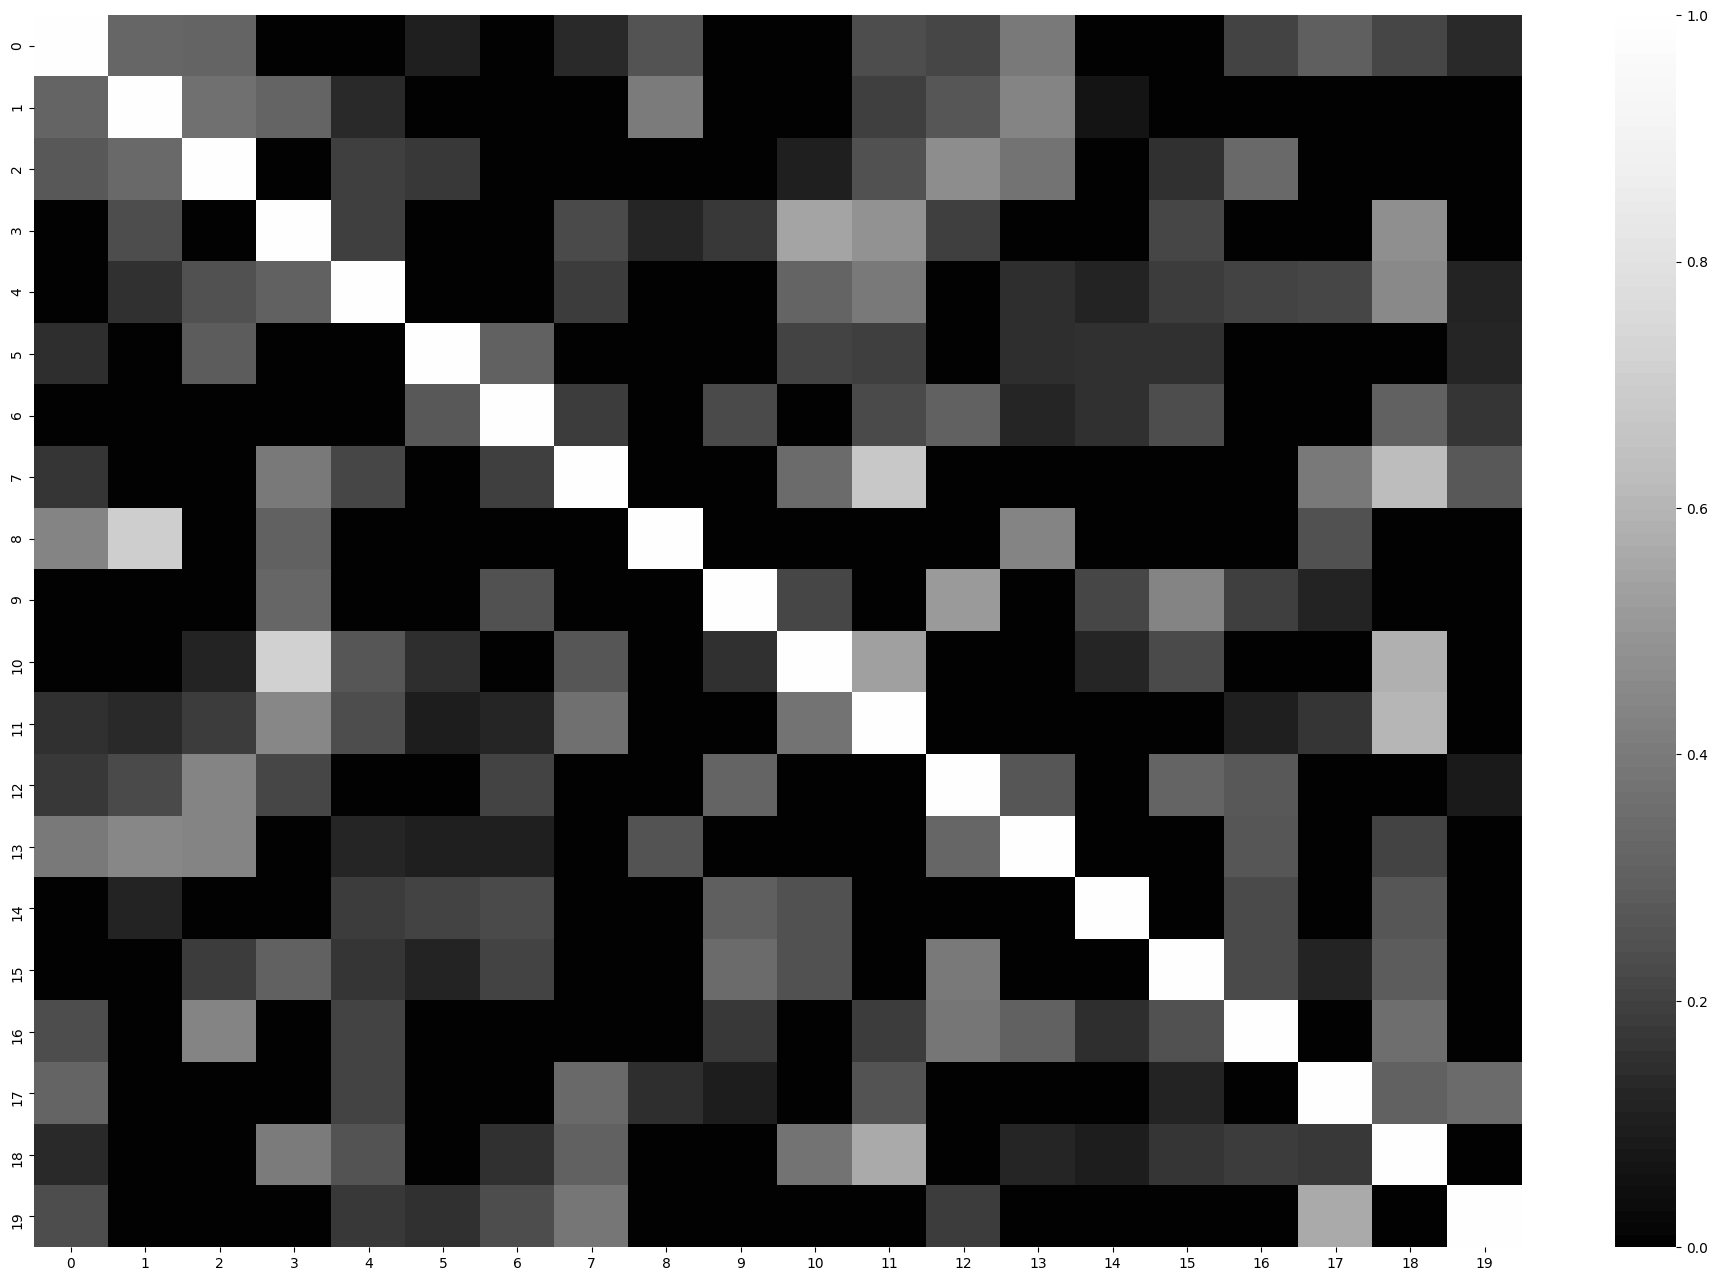
\includegraphics[width=\linewidth / 2]{figures/experiments/syn/20ng/MOA_relationship_graph.png}
	\caption[Relación entre etiquetas para cada \textit{stream} generado sobre
		la colección 20ng.]{Relación entre etiquetas para cada \textit{stream}
		generado sobre la colección 20ng. Arriba a la izquierda: \textit{Stream}
		original. Arriba a la derecha:\@ \textit{Stream} JC.\@ Abajo a la izquierda:\@
		\textit{Stream} JC\_BIG.\@ Abajo a la derecha:\@ \textit{Stream} MOA.}
	\label{fig:syn_20ng_label_relationship}
\end{figure}

La figura~\ref{fig:syn_20ng_label_relationship} es una representación visual de
la dependencia entre etiquetas. Ambos ejes del gráfico constan de las etiquetas
de la colección y cuánto mayor es la magnitud de color en la celda (en un rango
desde amarillo a rojo), mayor es la dependencia entre las dos etiquetas. Para
20ng los gráficos de la colección original, JC y JC\_BIG, son casi idénticos
entre sí por lo que es posible aseverar que el uso de la matriz de correlaciones
en la generación de \textit{streams} sintéticos ha contribuido a reproducir el
fenómeno de la dependencia entre etiquetas para esta colección.

\begin{table}[htbp]
	\centering
	\begin{adjustbox}{max width=\textwidth}
		\begin{tabular}{lllllllll}
	\toprule
	{}            & \multicolumn{2}{l}{20ng} & \multicolumn{2}{l}{JC} & \multicolumn{2}{l}{JC\_BIG} & \multicolumn{2}{l}{MOA}                                          \\
	\textit{Rank} & Atributo                 & Peso                   & Atributo
	              & Peso                     & Atributo               & Peso                        & Atributo                & Peso                                   \\
	\midrule
	1             & writes                   & 10116                  & source                      & 13590.5                 & source   & 56503.2 & bad     & 12178.6 \\[3pt]
	2             & article                  & 8715                   & issue                       & 13267.3                 & issue    & 54918   & koresh  & 10388.4 \\[3pt]
	3             & don                      & 5654                   & mouse                       & 13124.9                 & mouse    & 54359   & mass    & 9980.54 \\[3pt]
	4             & 1                        & 4790                   & site                        & 13037.3                 & site     & 53926.3 & school  & 9916.83 \\[3pt]
	5             & 2                        & 4314                   & food                        & 12971.7                 & food     & 53915.4 & widget  & 9836.48 \\[3pt]
	6             & people                   & 4258                   & model                       & 12888.9                 & bit      & 53534.8 & btw     & 9798.25 \\[3pt]
	7             & time                     & 4004                   & bit                         & 12885.9                 & model    & 53472.3 & smith   & 9767.02 \\[3pt]
	8             & good                     & 3727                   & muslim                      & 12880.4                 & decision & 53427.4 & provide & 9765.89 \\[3pt]
	9             & make                     & 3231                   & decision                    & 12858.8                 & happened & 53165.4 & issues  & 9762.76 \\[3pt]
	10            & 3                        & 3212                   & happened                    & 12824.2                 & good     & 52918.9 & faith   & 9756.81 \\
	\bottomrule
\end{tabular}



	\end{adjustbox}
	\caption{Espacio de atributos para \textit{streams} 20ng.}
	\label{tab:syn_20ng_features_space}
\end{table}

Finalmente, la figura~\ref{tab:syn_20ng_features_space} lista los atributos más
frecuentes de cada \textit{stream} y da una idea del espacio de atributos
generado.

\subsubsection{Enron}

\begin{table}[htbp]
	\centering
	\begin{adjustbox}{max width=\textwidth}
		\begin{tabular}{lrrrr}
	\toprule
	\multicolumn{5}{c}{Enron}             \\
	Nombre  & N      & L  & LC    & LD    \\
	\midrule
	Enron   & 1702   & 53 & 3,378 & 0,064 \\
	MOA     & 1702   & 53 & 3,707 & 0,070 \\
	JC      & 1702   & 53 & 2,330 & 0,044 \\
	JC\_BIG & 100000 & 53 & 2,321 & 0,044 \\
	\bottomrule
\end{tabular}

	\end{adjustbox}
	\caption[Características de los \textit{streams} sintéticos generados sobre
		la colección Enron.]{Características de los \textit{streams} sintéticos
		generados sobre la colección Enron.  N:\@ número de instancias; L:\@
		número de etiquetas; LC:\@ cardinalidad de etiquetas; LD:\@ densidad de
		etiquetas.}
	\label{tab:syn_enron_stats}
\end{table}

\begin{figure}[htbp]
	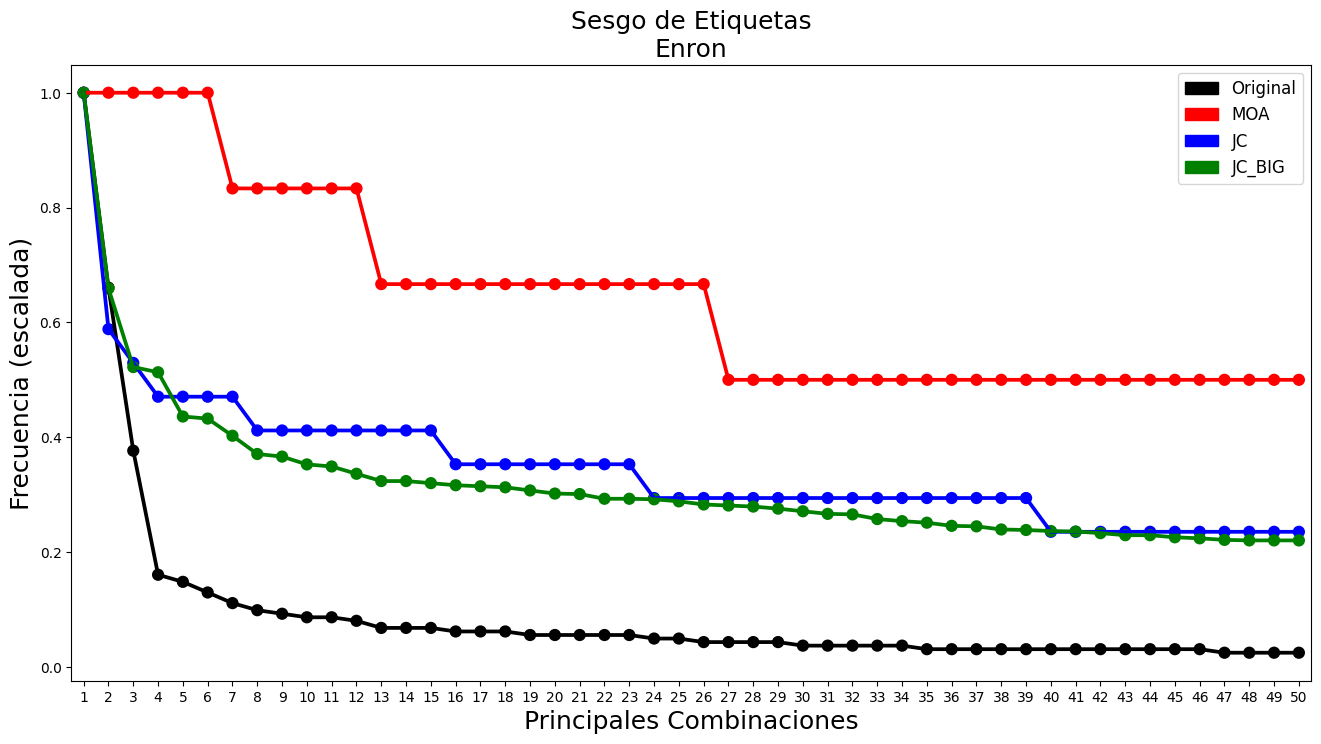
\includegraphics[width=\linewidth]{figures/experiments/syn/enron/label_skew.png}
	\caption{Sesgo de etiquetas de los \textit{streams} generados sobre la colección
		Enron.}
	\label{fig:syn_enron_label_skew}
\end{figure}

\begin{table}[htbp]
	\centering
	\begin{adjustbox}{max width=\textwidth}
		\begin{tabular}{lllll}
	\toprule
	\textit{Rank} & Original             & JC               & JC\_BIG          & MOA                           \\
	\midrule
	1             & \{A.A4\}             & \{A.A4, C.C13\}  & \{A.A4, C.C13\}  & \{B.B12, B.B4, D.D10, C.C1\}  \\
	2             & \{B.B2, A.A4, B.B1\} & \{C.C10, D.D18\} & \{A.A6, D.D18\}  & \{D.D1, A.A5, D.D5, B.B10\}   \\
	3             & \{B.B2, A.A4\}       & \{A.A4, D.D4\}   & \{C.C10, D.D18\} & \{A.A8, B.B3, D.D16, B.B9\}   \\
	4             & \{A.A1, B.B4, C.C6\} & \{A.A7, B.B13\}  & \{A.A7, B.B13\}  & \{C.C7, D.D13, D.D10, D.D18\} \\
	5             & \{B.B2, A.A5, B.B1\} & \{A.A4, B.B9\}   & \{A.A1, D.D18\}  & \{C.C5, B.B2, A.A6, D.D15\}   \\
	\bottomrule
\end{tabular}


	\end{adjustbox}
	\caption{Sesgo de etiquetas: Principales combinaciones de los
		\textit{streams} generados sobre la colección Enron.}
	\label{tab:syn_enron_top_labels_combinations}
\end{table}

Partiendo de la tabla~\ref{tab:syn_enron_stats} se observa que el
\textit{stream} MOA se aproxima más al valor de cardinalidad de la colección
original que nuestra propuesta. Sin embargo, JC Y JC\_BIG, describen una curva
en el gráfico de la figura~\ref{fig:syn_enron_label_skew} que, en comparación
con MOA, tiene una mayor similitud con la curva de la colección original.  Se
adjunta la tabla~\ref{tab:syn_enron_top_labels_combinations} como complemento al
estudio del sesgo.

\begin{figure}[htbp]
	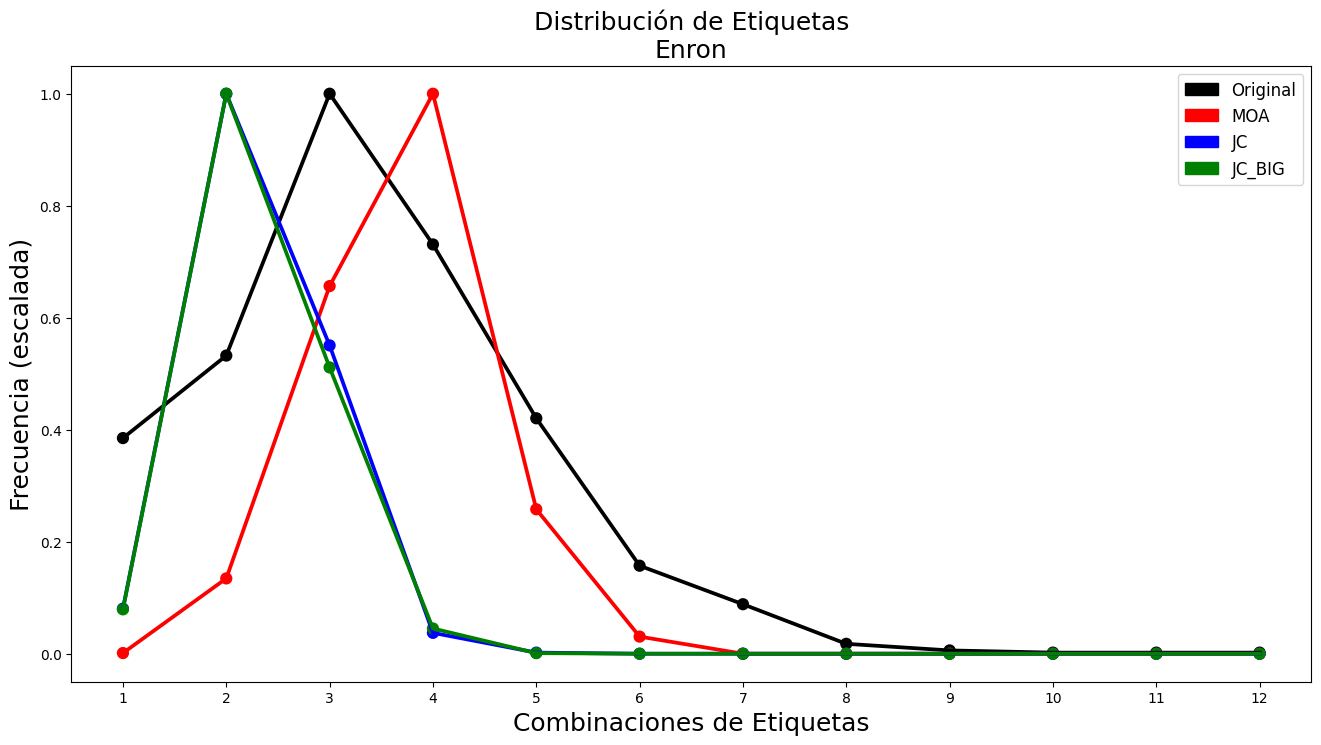
\includegraphics[width=\linewidth]{figures/experiments/syn/enron/label_distribution.png}
	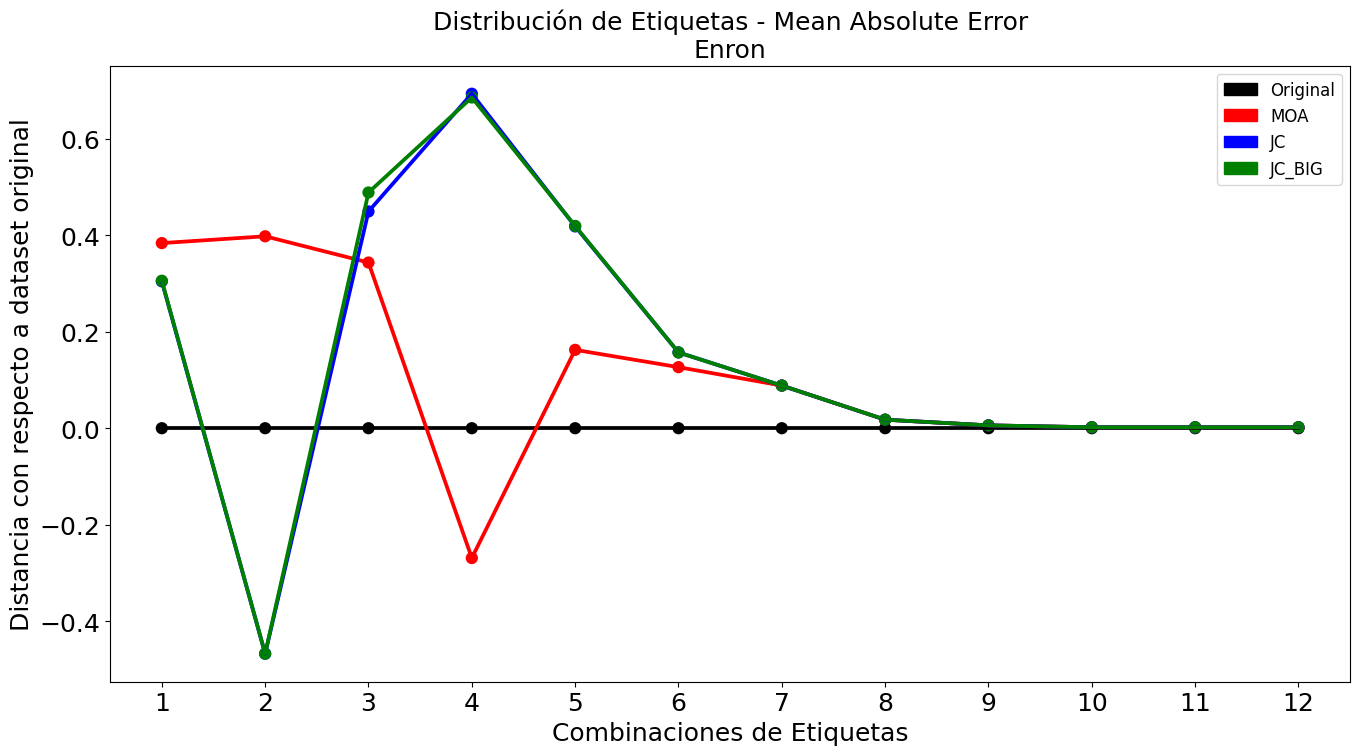
\includegraphics[width=\linewidth]{figures/experiments/syn/enron/ld_mae.png}
	\caption[Distribución de etiquetas de los \textit{streams} generados sobre la colección
		Enron.]{Distribución de etiquetas de los \textit{streams} generados sobre la colección
		Enron. Arriba se encuentra el gráfico con las frecuencias escaladas y
		abajo el \textit{mean absolute error} entre cada \textit{stream} y la
		colección original.}
	\label{fig:syn_enron_label_distribution}
\end{figure}

Con respecto a la distribución de etiquetas
(figura~\ref{fig:syn_enron_label_distribution}) no es posible determinar si
alguno de los \textit{streams} refleja el fenómeno en mayor grado que otro. Al
mismo tiempo, si bien ninguno de ellos logra reproducir con exactitud la
composición de la cardinalidad entre conjuntos de etiquetas, hay un grado de
similitud entre curvas (ver gráfico de \textit{mean absolute error}) que podría
ser aceptable, dependiendo de la tarea a resolver. En cuanto al tipo de
distribución, del cual se hace mención en el trabajo de referencia, todos los
\textit{streams} sintéticos obedecen al tipo B, es decir, la mayoría de los
ejemplos tienen una cardinalidad de etiquetas mayor que uno.

\begin{figure}[htbp]
	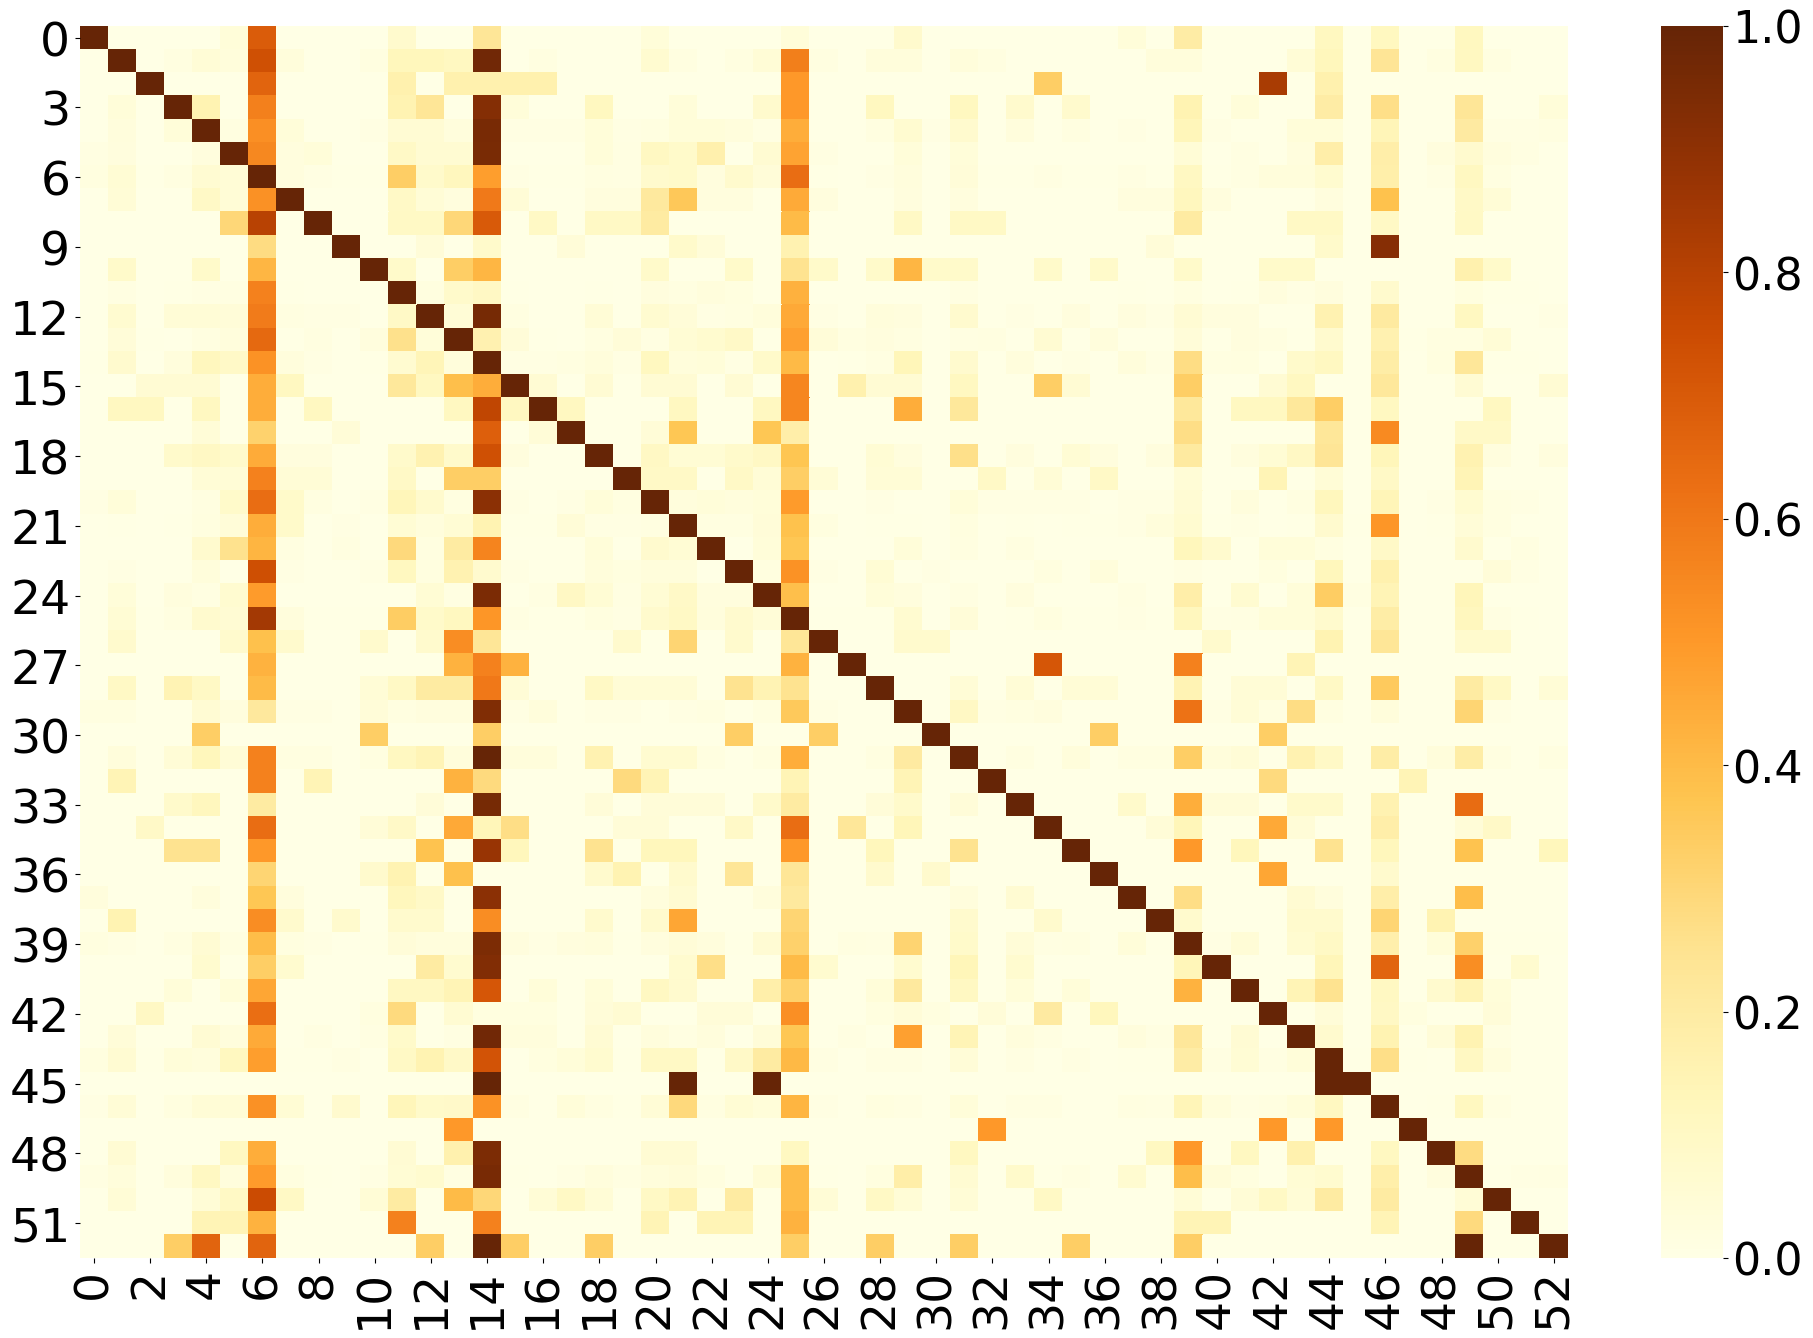
\includegraphics[width=\linewidth / 2]{figures/experiments/syn/enron/enron_relationship_graph.png}
	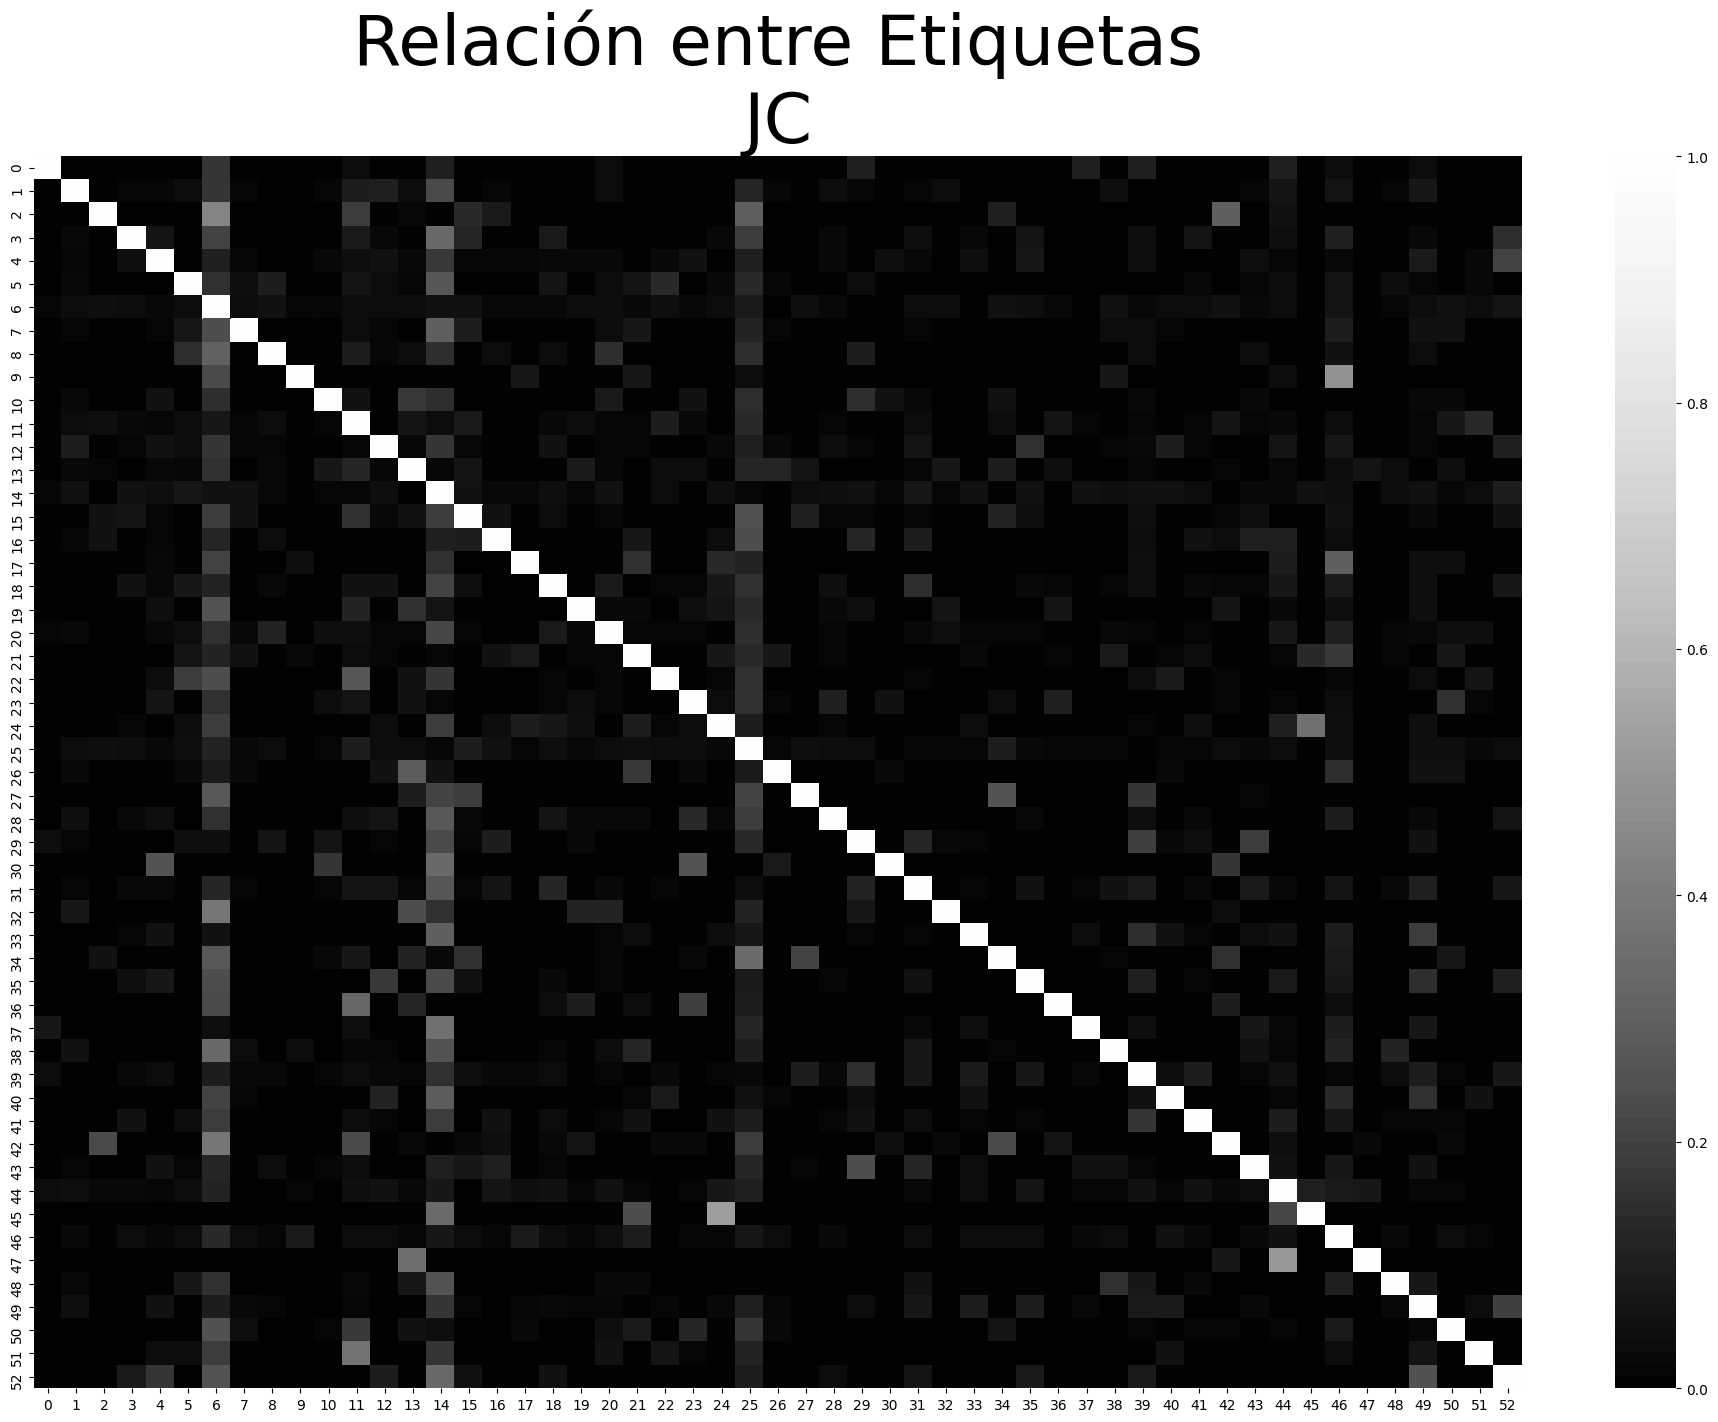
\includegraphics[width=\linewidth /
		2]{figures/experiments/syn/enron/JC_relationship_graph.png}
	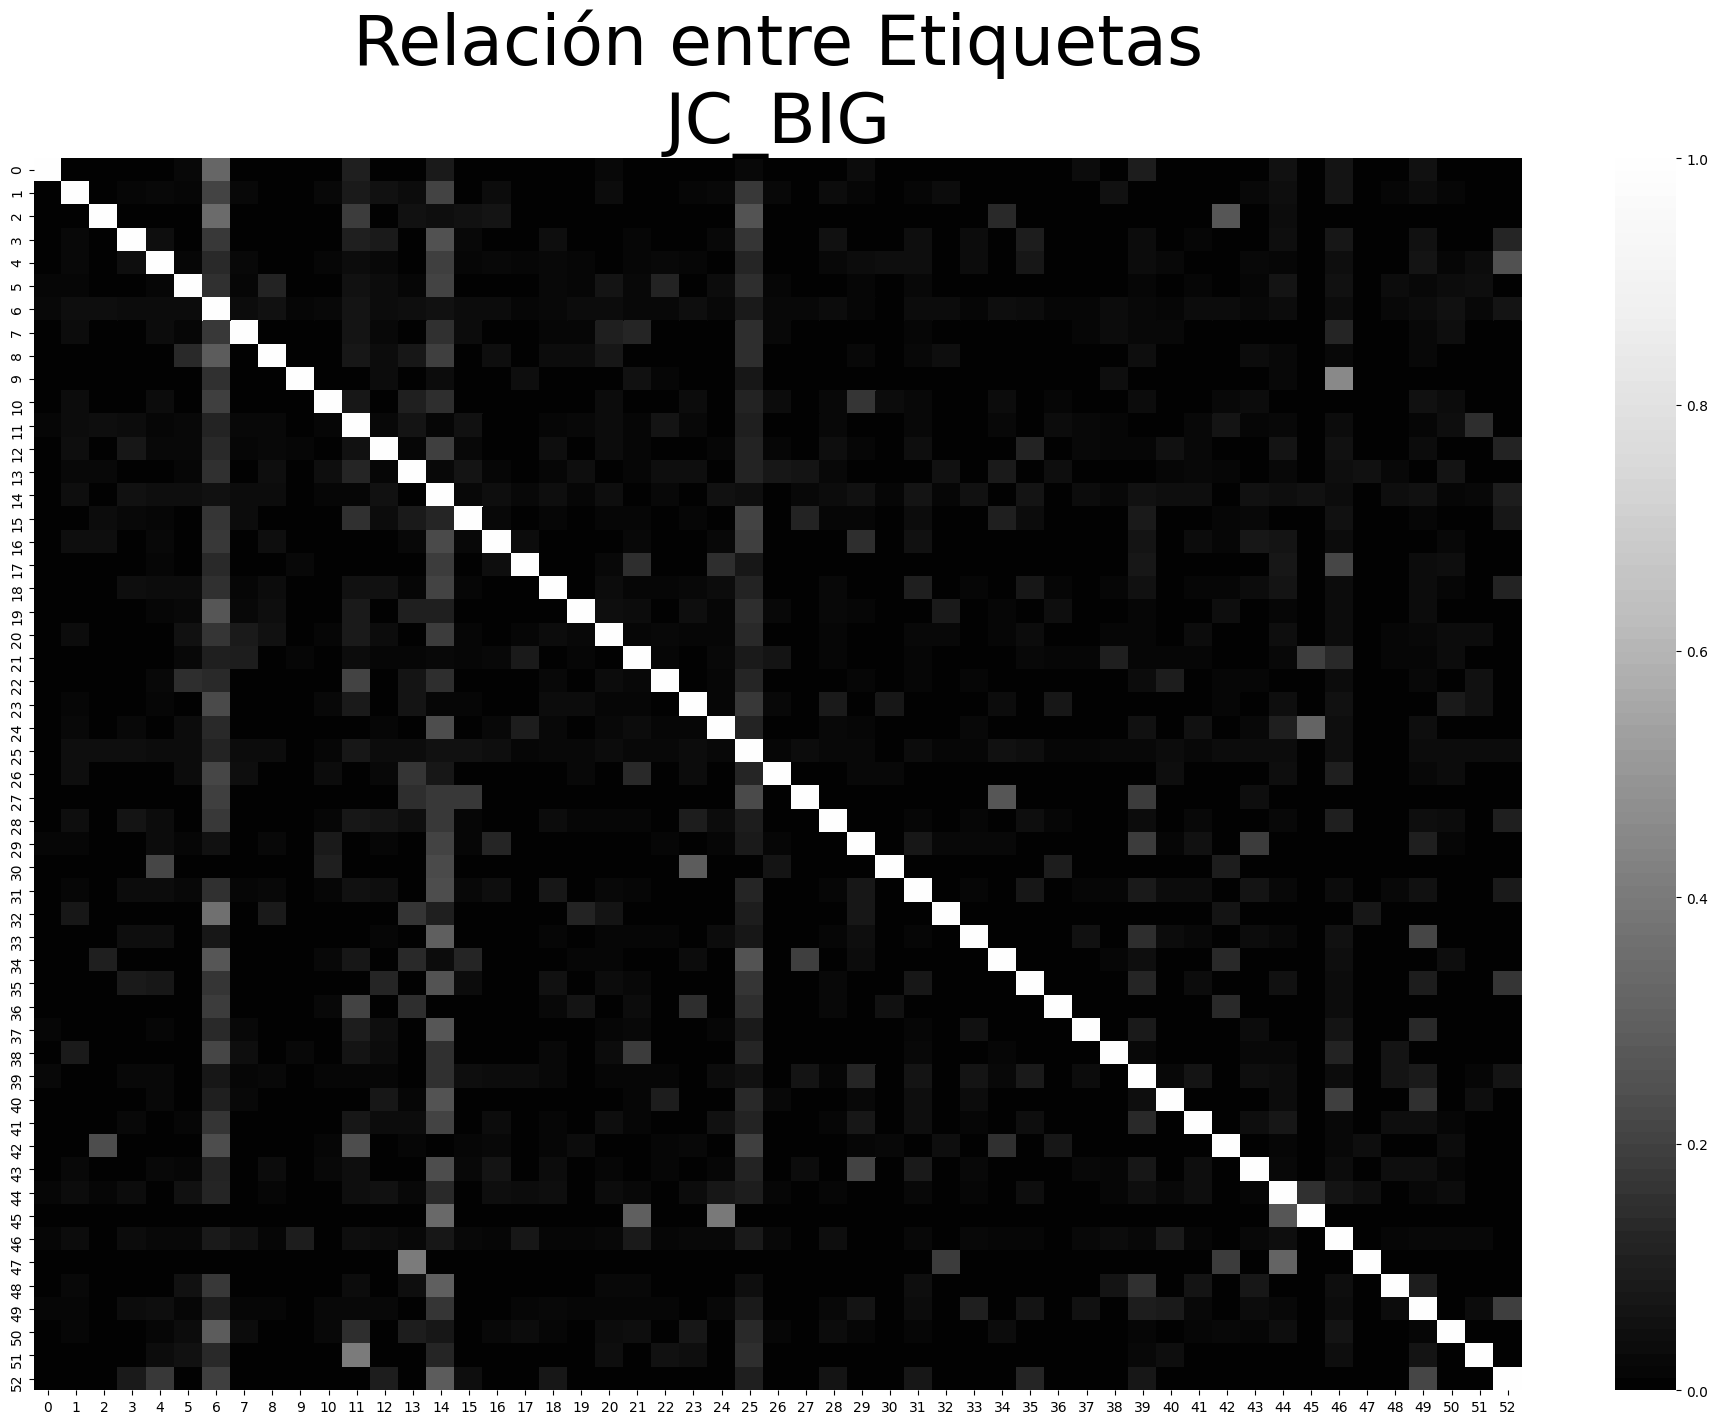
\includegraphics[width=\linewidth /
		2]{figures/experiments/syn/enron/JC_BIG_relationship_graph.png}
	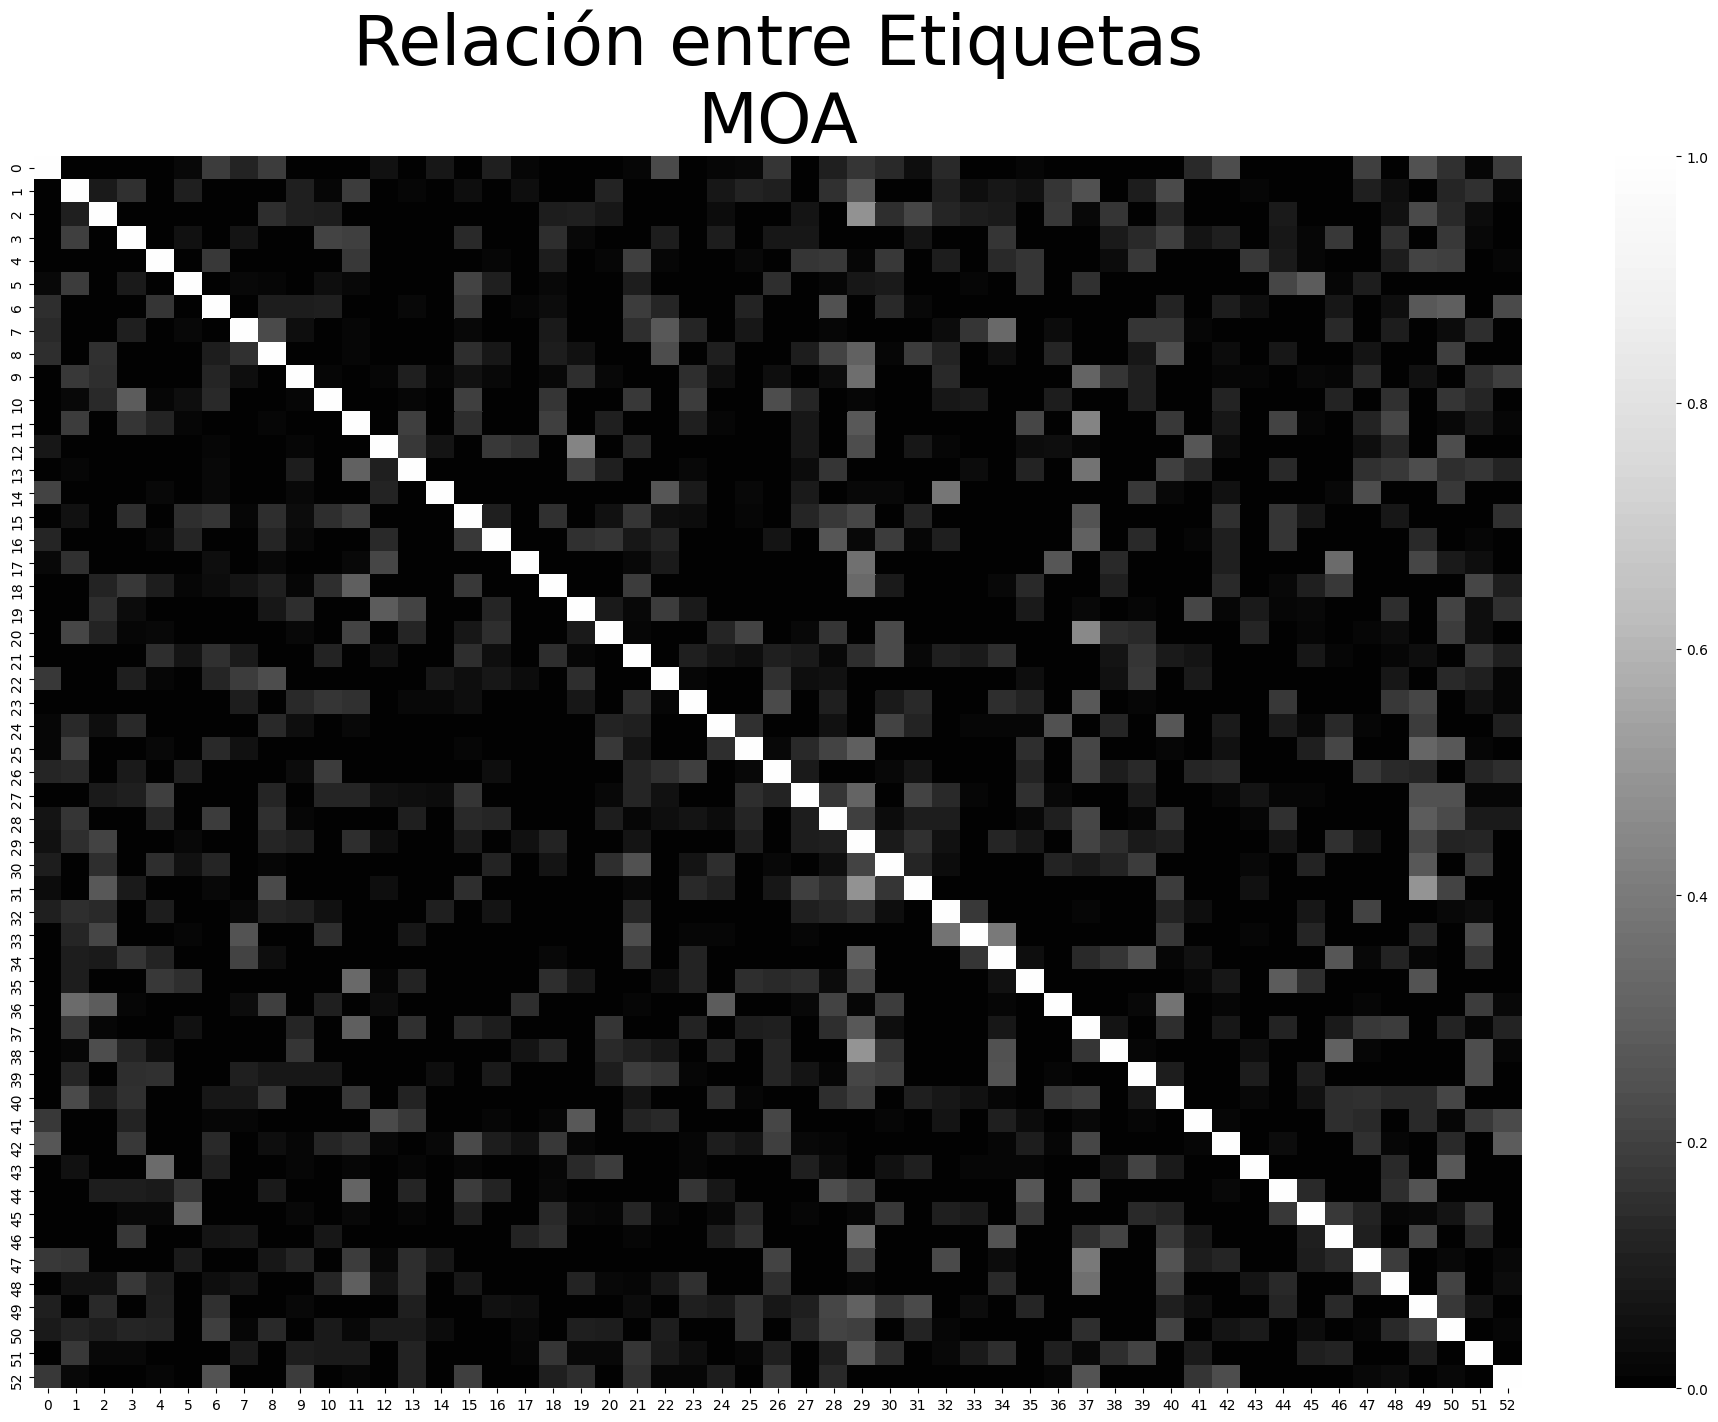
\includegraphics[width=\linewidth /
		2]{figures/experiments/syn/enron/MOA_relationship_graph.png}
	\caption[Relación entre etiquetas para cada \textit{stream} generado sobre
		la colección Enron.]{Relación entre etiquetas para cada \textit{stream} generado sobre
		la colección Enron. Arriba a la izquierda: \textit{Stream} original. Arriba a la
		derecha: \textit{Stream} JC.\@ Abajo a la izquierda: \textit{Stream}
		JC\_BIG.\@ Abajo a la derecha: \textit{Stream} MOA.}
	\label{fig:syn_enron_label_relationship}
\end{figure}

Por otro lado, el fenómeno de la dependencia entre etiquetas es representado
visualmente por la figura~\ref{fig:syn_enron_label_relationship}. Tal como
sucedió con la colección 20ng, los gráficos de JC y JC\_BIG para Enron reflejan
una coloración muy similar al del original, aunque con una tonalidad de blanco
menos intensa. Este comportamiento podría estar emparentado con la cardinalidad
de etiquetas, que en estos \textit{streams} sintéticos es menor. No obstante, se
requieren más estudios para arribar a una conclusión al respecto.

\begin{table}[htbp]
	\centering
	\begin{adjustbox}{max width=\textwidth}
		\begin{tabular}{lllllllll}
	\toprule
	{}            & \multicolumn{2}{l}{enron} & \multicolumn{2}{l}{JC} & \multicolumn{2}{l}{JC\_BIG} & \multicolumn{2}{l}{MOA}                                              \\
	\textit{Rank} & Atributo                  & Peso                   & Atributo                    & Peso                    & Atributo & Peso    & Atributo    & Peso    \\
	\midrule
	1             & enron                     & 1186                   & cut                         & 1238.8                  & cut      & 73252.8 & past        & 1086.29 \\[3pt]
	2             & subject                   & 1057                   & capacity                    & 1190.77                 & capacity & 70263.5 & real        & 934.726 \\[3pt]
	3             & 2001                      & 856                    & seeking                     & 1189.24                 & run      & 69067.8 & legislature & 893.989 \\[3pt]
	4             & steven                    & 776                    & run                         & 1172.62                 & bonds    & 68871.9 & calif       & 892.211 \\[3pt]
	5             & kean                      & 772                    & bonds                       & 1169.24                 & seeking  & 68673.9 & settlement  & 887.738 \\[3pt]
	6             & forwarded                 & 681                    & efforts                     & 1169.22                 & efforts  & 68102.1 & agency      & 886.591 \\[3pt]
	7             & na                        & 659                    & 90                          & 1154.21                 & 90       & 67915.7 & addition    & 883.931 \\[3pt]
	8             & pmto                      & 580                    & remains                     & 1150.76                 & problem  & 67029.4 & 10          & 883.781 \\[3pt]
	9             & pm                        & 567                    & problem                     & 1139.46                 & remains  & 66706.4 & diego       & 883.126 \\[3pt]
	10            & 10                        & 558                    & big                         & 1135.77                 & big      & 66353.7 & spent       & 882.981 \\
	\bottomrule
\end{tabular}



	\end{adjustbox}
	\caption{Espacio de atributos para \textit{streams} Enron.}
	\label{tab:syn_enron_features_space}
\end{table}

Por último, la figura~\ref{tab:syn_enron_features_space} lista los atributos más
frecuentes de cada \textit{stream} y da una idea del espacio de atributos
generado.

\subsubsection{Mediamill}

\begin{table}[htbp]
	\centering
	\begin{adjustbox}{max width=\textwidth}
		\begin{tabular}{lrrrr}
	\toprule
	\multicolumn{5}{c}{Mediamill}            \\[3pt]
	Nombre    & N      & L   & LC    & LD    \\
	\midrule
	Mediamill & 43907  & 101 & 4,376 & 0,043 \\[3pt]
	MOA       & 43907  & 101 & 4,071 & 0,040 \\[3pt]
	JC        & 43907  & 101 & 2,435 & 0,024 \\[3pt]
	JC\_BIG   & 500000 & 101 & 2,439 & 0,024 \\
	\bottomrule
\end{tabular}

	\end{adjustbox}
	\caption[Características de los \textit{streams} sintéticos generados sobre
		la colección Mediamill.]{Características de los \textit{streams}
		sintéticos generados sobre la colección Mediamill.  N:\@ número de
		instancias; L:\@ número de etiquetas; LC:\@ cardinalidad de etiquetas; LD:\@
		densidad de etiquetas.}
	\label{tab:syn_mediamill_stats}
\end{table}

\begin{figure}[htbp]
	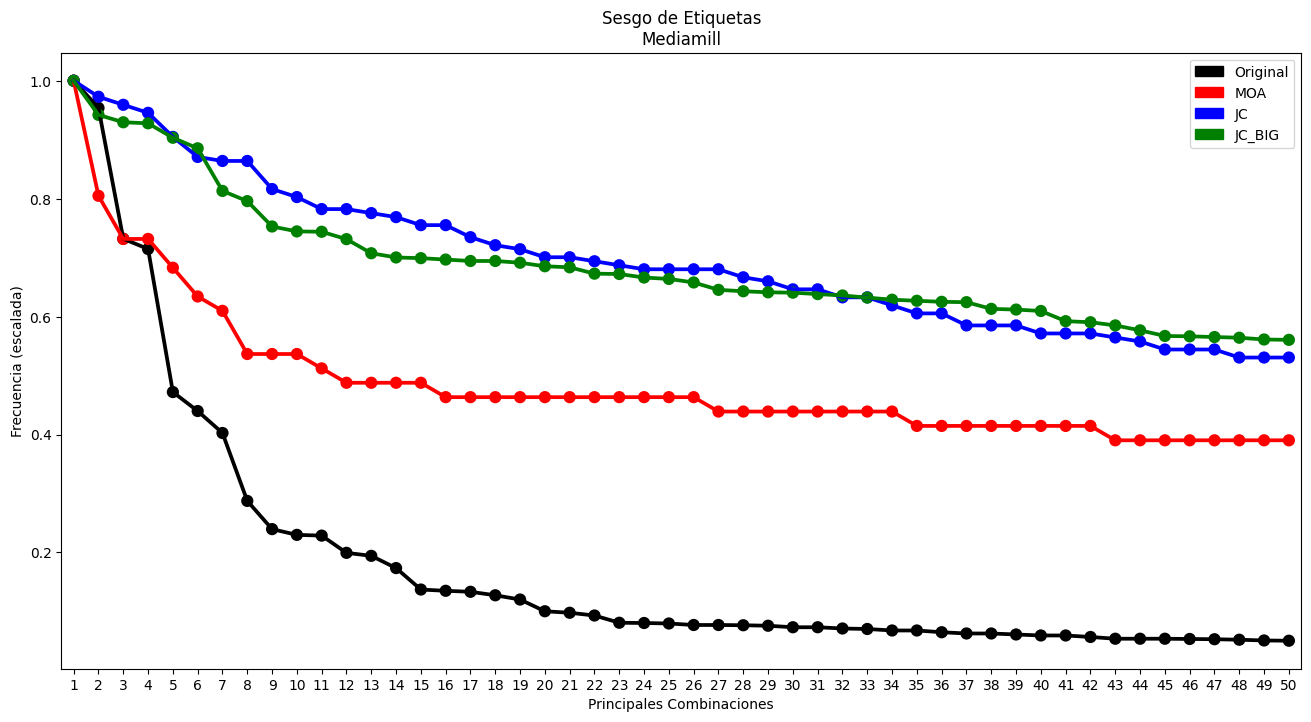
\includegraphics[width=\linewidth]{figures/experiments/syn/mediamill/label_skew.png}
	\caption{Sesgo de etiquetas de los \textit{streams} generados sobre la
		colección Mediamill.}
	\label{fig:syn_mediamill_label_skew}
\end{figure}

\begin{table}[htbp]
	\centering
	\begin{adjustbox}{max width=\textwidth}
		\begin{tabular}{lllll}
	\toprule
	\textit{Rank} & Original                      & JC                            & JC\_BIG                       & MOA                                             \\
	\midrule
	1             & \{Class32, Class34, Class68\} & \{Class48, Class49, Class68\} & \{Class3, Class85\}           & \{Class32, Class38, Class50, Class72\}          \\[3pt]
	2             & \{Class34, Class68\}          & \{Class63, Class85\}          & \{Class31, Class85\}          & \{Class3, Class26, Class89\}                    \\[3pt]
	3             & \{\}                          & \{Class31, Class85\}          & \{Class83, Class85\}          & \{Class18, Class34, Class35, Class89\}          \\[3pt]
	4             & \{Class67\}                   & \{Class3, Class85\}           & \{Class63, Class85\}          & \{Class34, Class35, Class42, Class50, Class73\} \\[3pt]
	5             & \{Class34, Class67, Class68\} & \{Class34, Class78\}          & \{Class32, Class48, Class49\} & \{Class34, Class35, Class42, Class50\}          \\
	\bottomrule
\end{tabular}


	\end{adjustbox}
	\caption{Sesgo de etiquetas: Principales combinaciones de los
		\textit{streams} generados sobre la colección Mediamill.}
	\label{tab:syn_mediamill_top_labels_combinations}
\end{table}

La tabla~\ref{tab:syn_mediamill_stats} muestra que el \textit{stream} MOA hace
un buen trabajo en aproximar la cardinalidad de la colección original y presenta
la curva de sesgo más cercana a ella (ver
figura~\ref{fig:syn_mediamill_label_skew}). Se adjunta la
tabla~\ref{tab:syn_20ng_top_labels_combinations} como complemento al estudio del
sesgo.

\begin{figure}[htbp]
	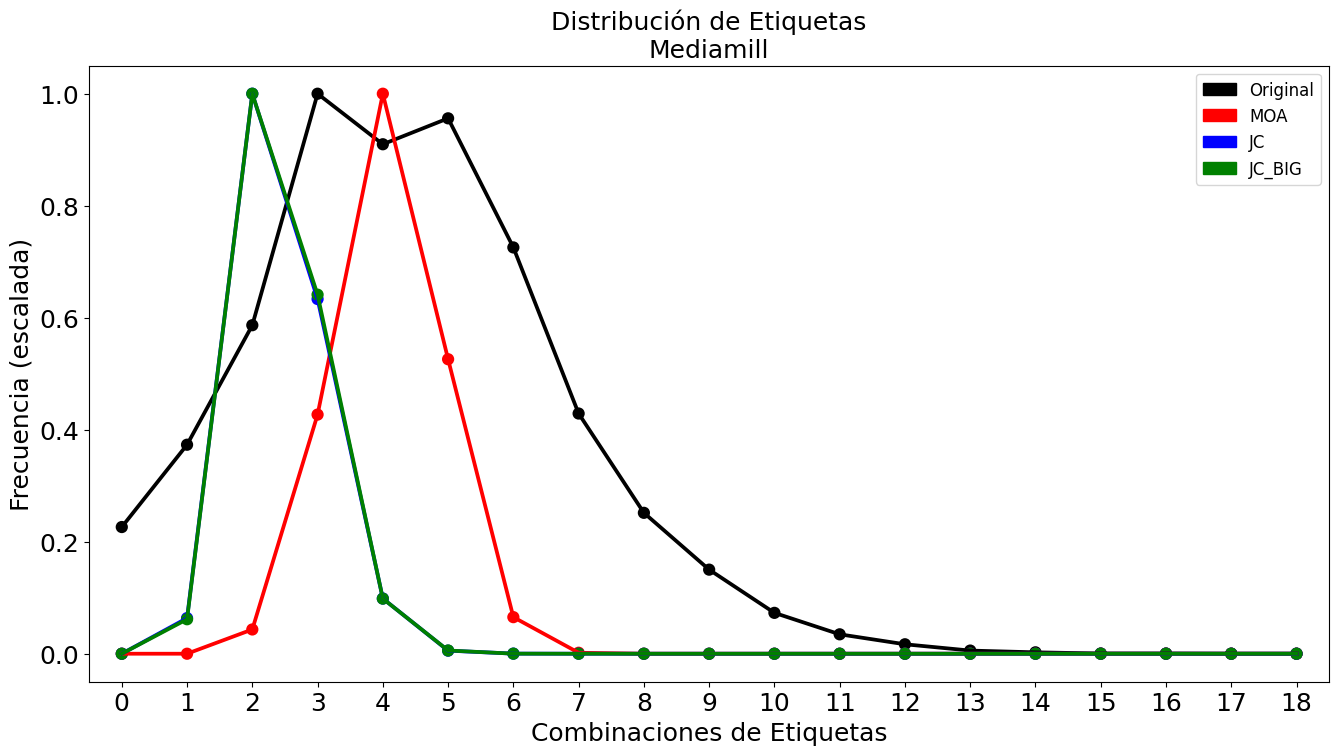
\includegraphics[width=\linewidth]{figures/experiments/syn/mediamill/label_distribution.png}
	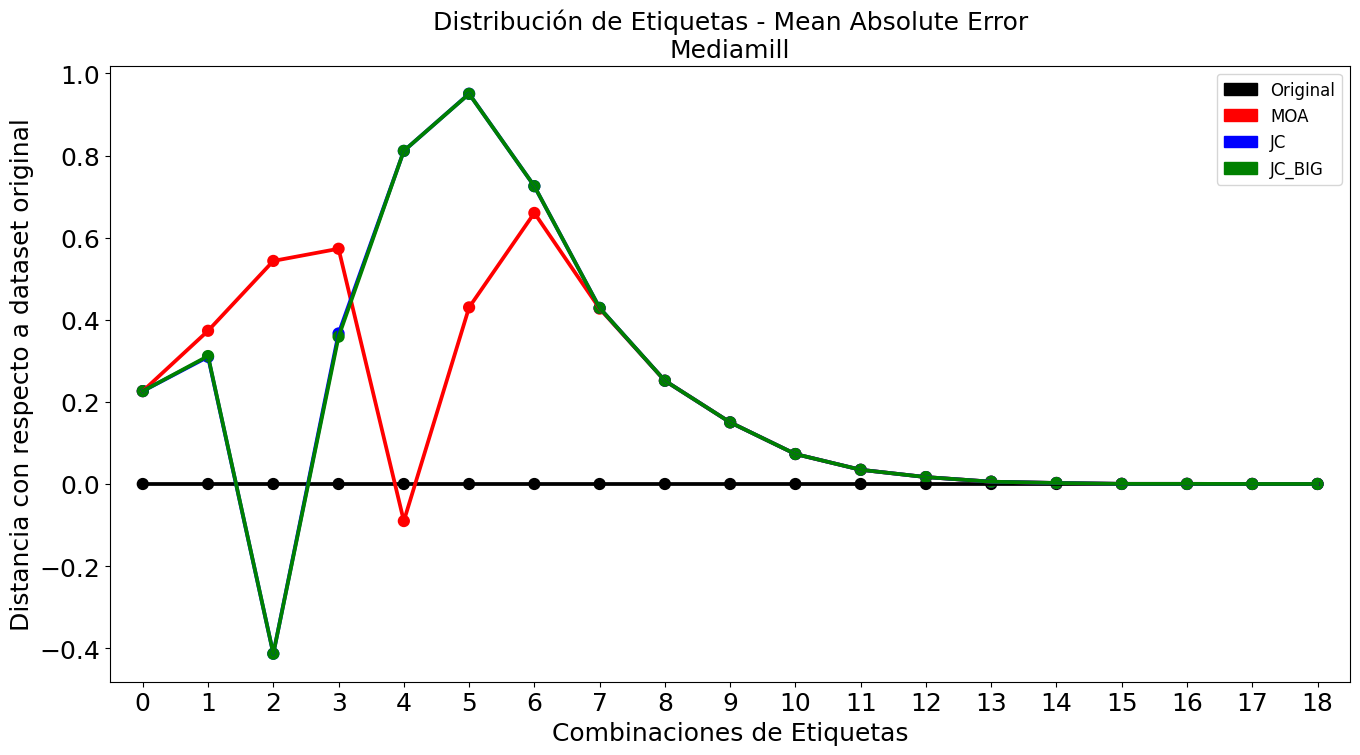
\includegraphics[width=\linewidth]{figures/experiments/syn/mediamill/ld_mae.png}
	\caption[Distribución de etiquetas de los \textit{streams} generados sobre la colección
		Mediamill.]{Distribución de etiquetas de los \textit{streams} generados sobre la colección
		Mediamill. Arriba se encuentra el gráfico con las frecuencias escaladas y
		abajo el \textit{mean absolute error} entre cada \textit{stream} y la
		colección original.}
	\label{fig:syn_mediamill_label_distribution}
\end{figure}

Con respecto a la distribución de etiquetas
(figura~\ref{fig:syn_mediamill_label_distribution}) las conclusiones son
similares a las realizadas a este efecto para Enron. No es posible determinar
con certeza que alguno de los \textit{streams} refleja el fenómeno en mayor
grado que otro, e incluso, si se analiza el gráfico de \textit{mean absolute
	error}, se puede observar que hay 3 puntos donde la curva de JC se aproxima más
al del original y 3 donde el más próximo es MOA.\@ En cuanto al tipo de
distribución, del cual se hace mención en el trabajo de referencia, todos los
\textit{streams} sintéticos obedecen al tipo B, es decir, la mayoría de los
ejemplos tienen una cardinalidad de etiquetas mayor que uno.

\begin{figure}[htbp]
	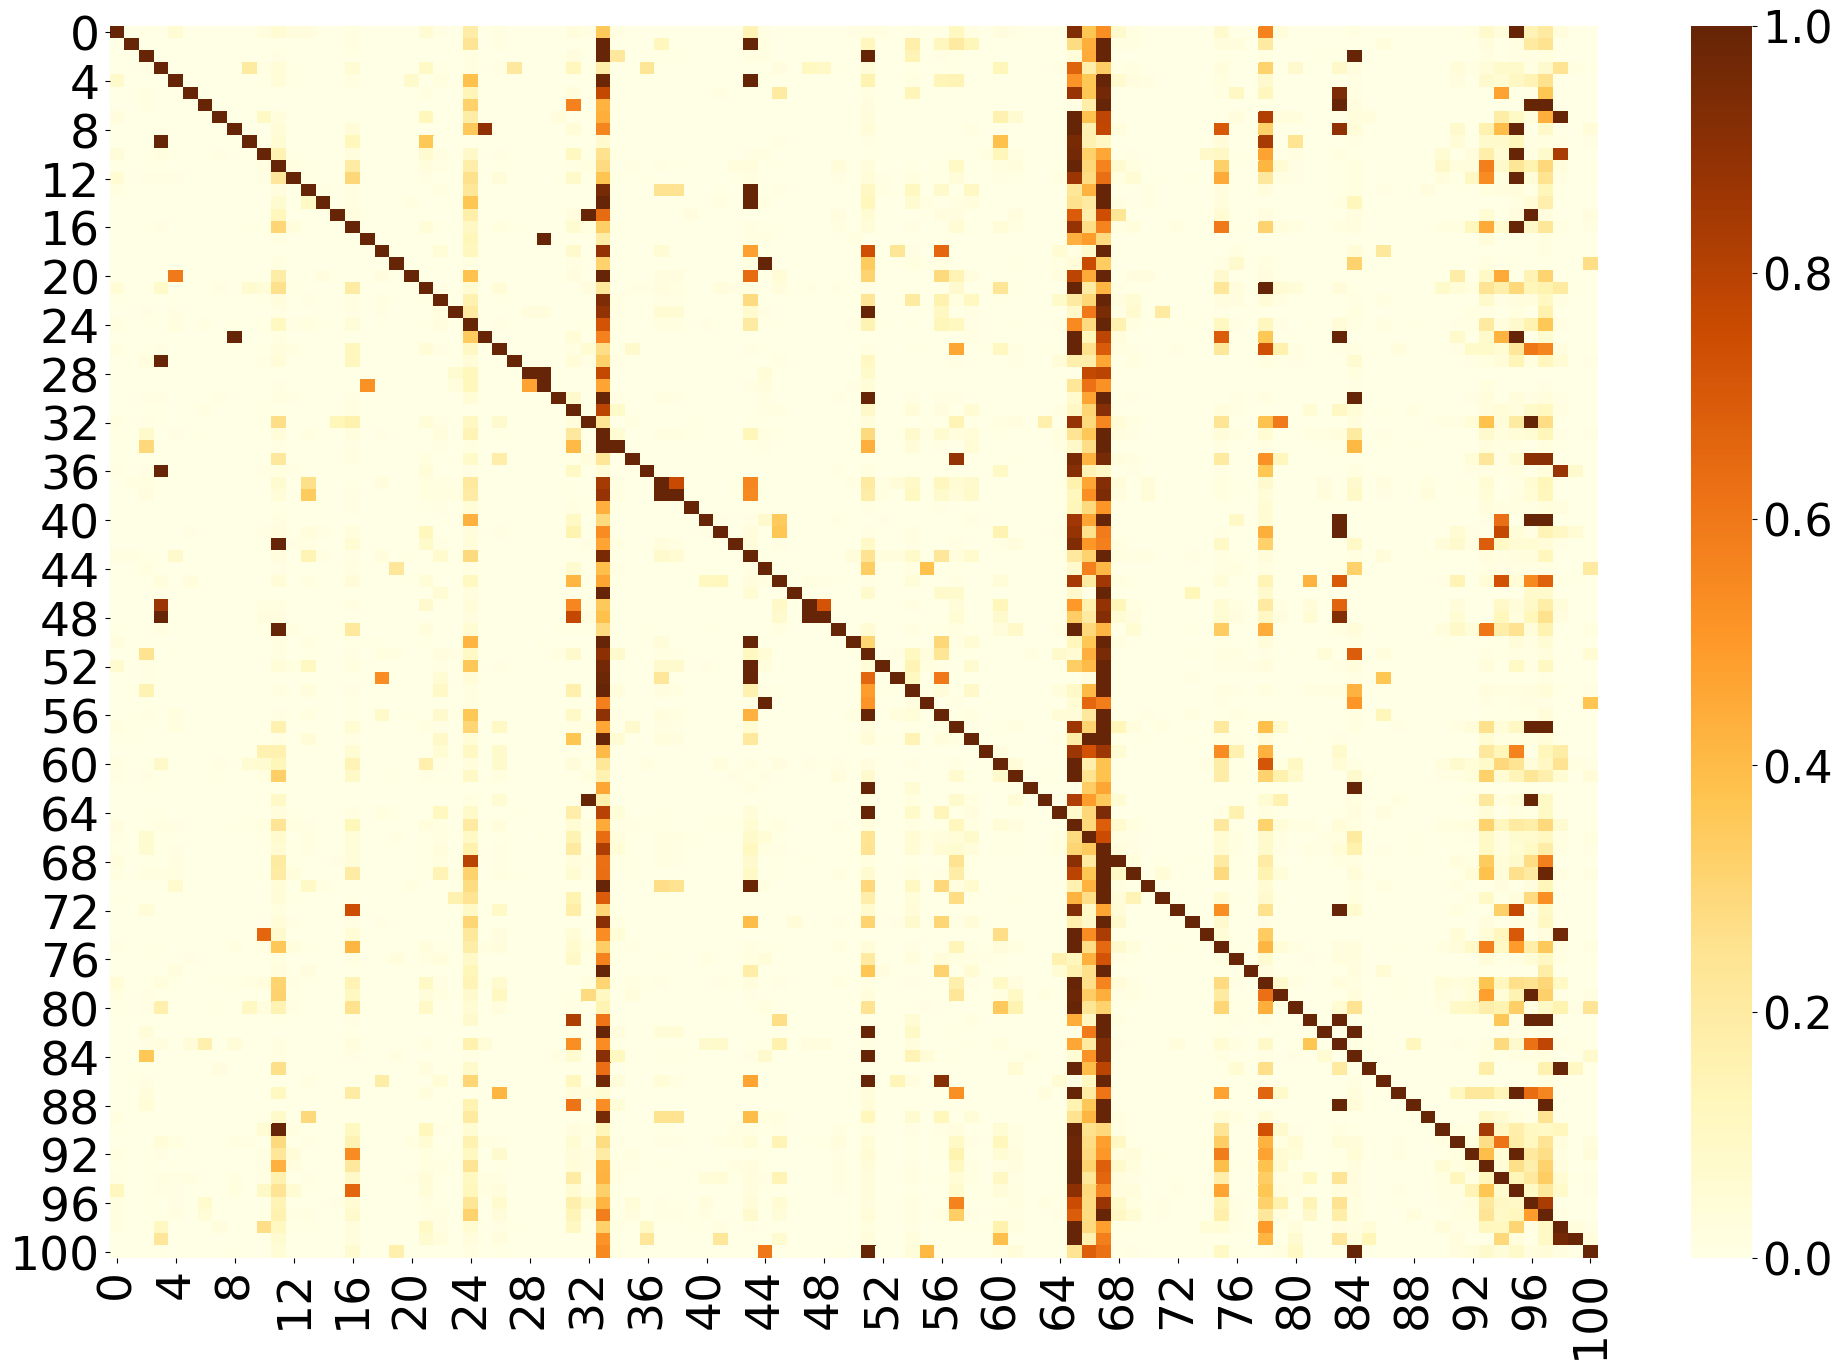
\includegraphics[width=\linewidth /
		2]{figures/experiments/syn/mediamill/mediamill_relationship_graph.png}
	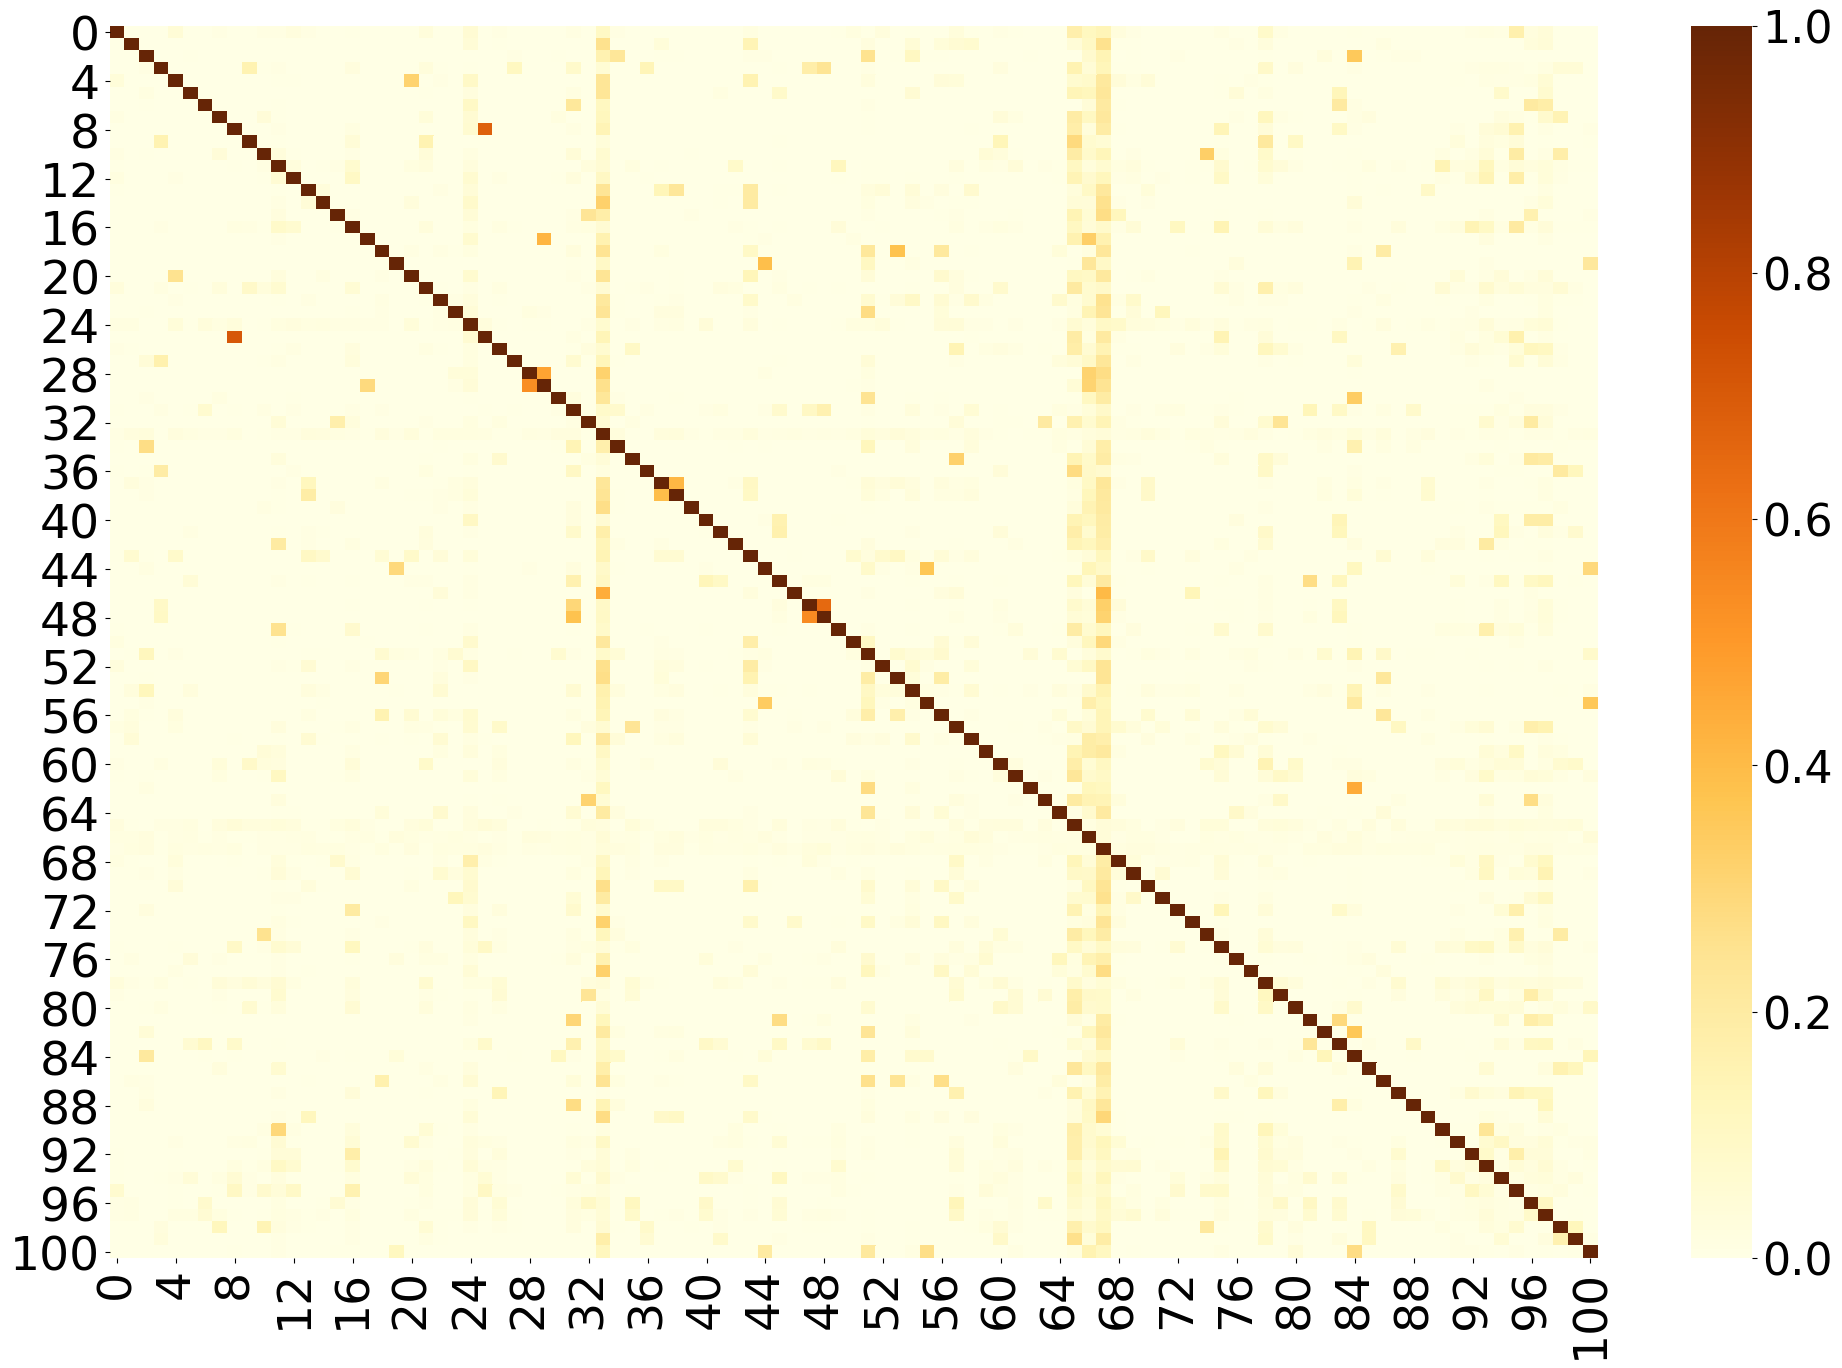
\includegraphics[width=\linewidth /
		2]{figures/experiments/syn/mediamill/JC_relationship_graph.png}
	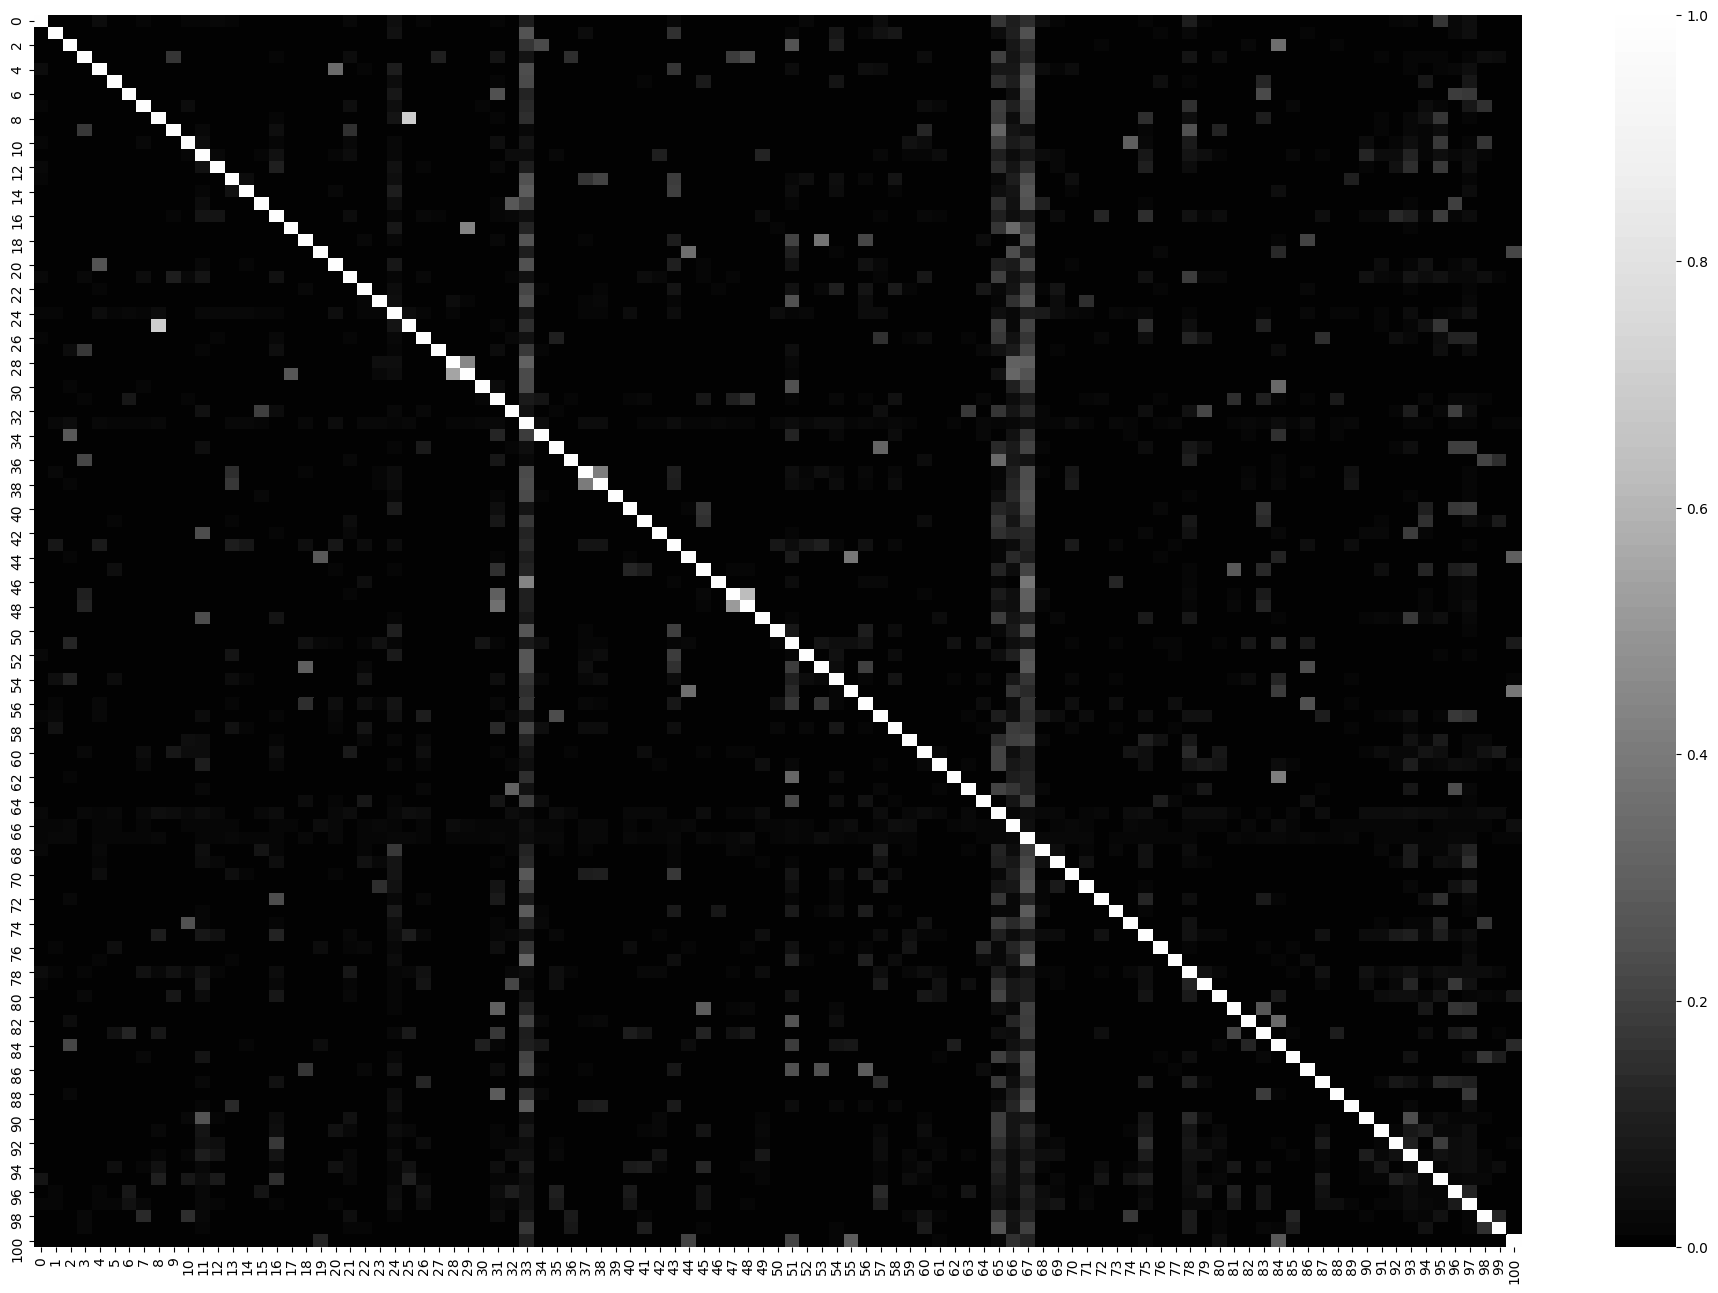
\includegraphics[width=\linewidth /
		2]{figures/experiments/syn/mediamill/JC_BIG_relationship_graph.png}
	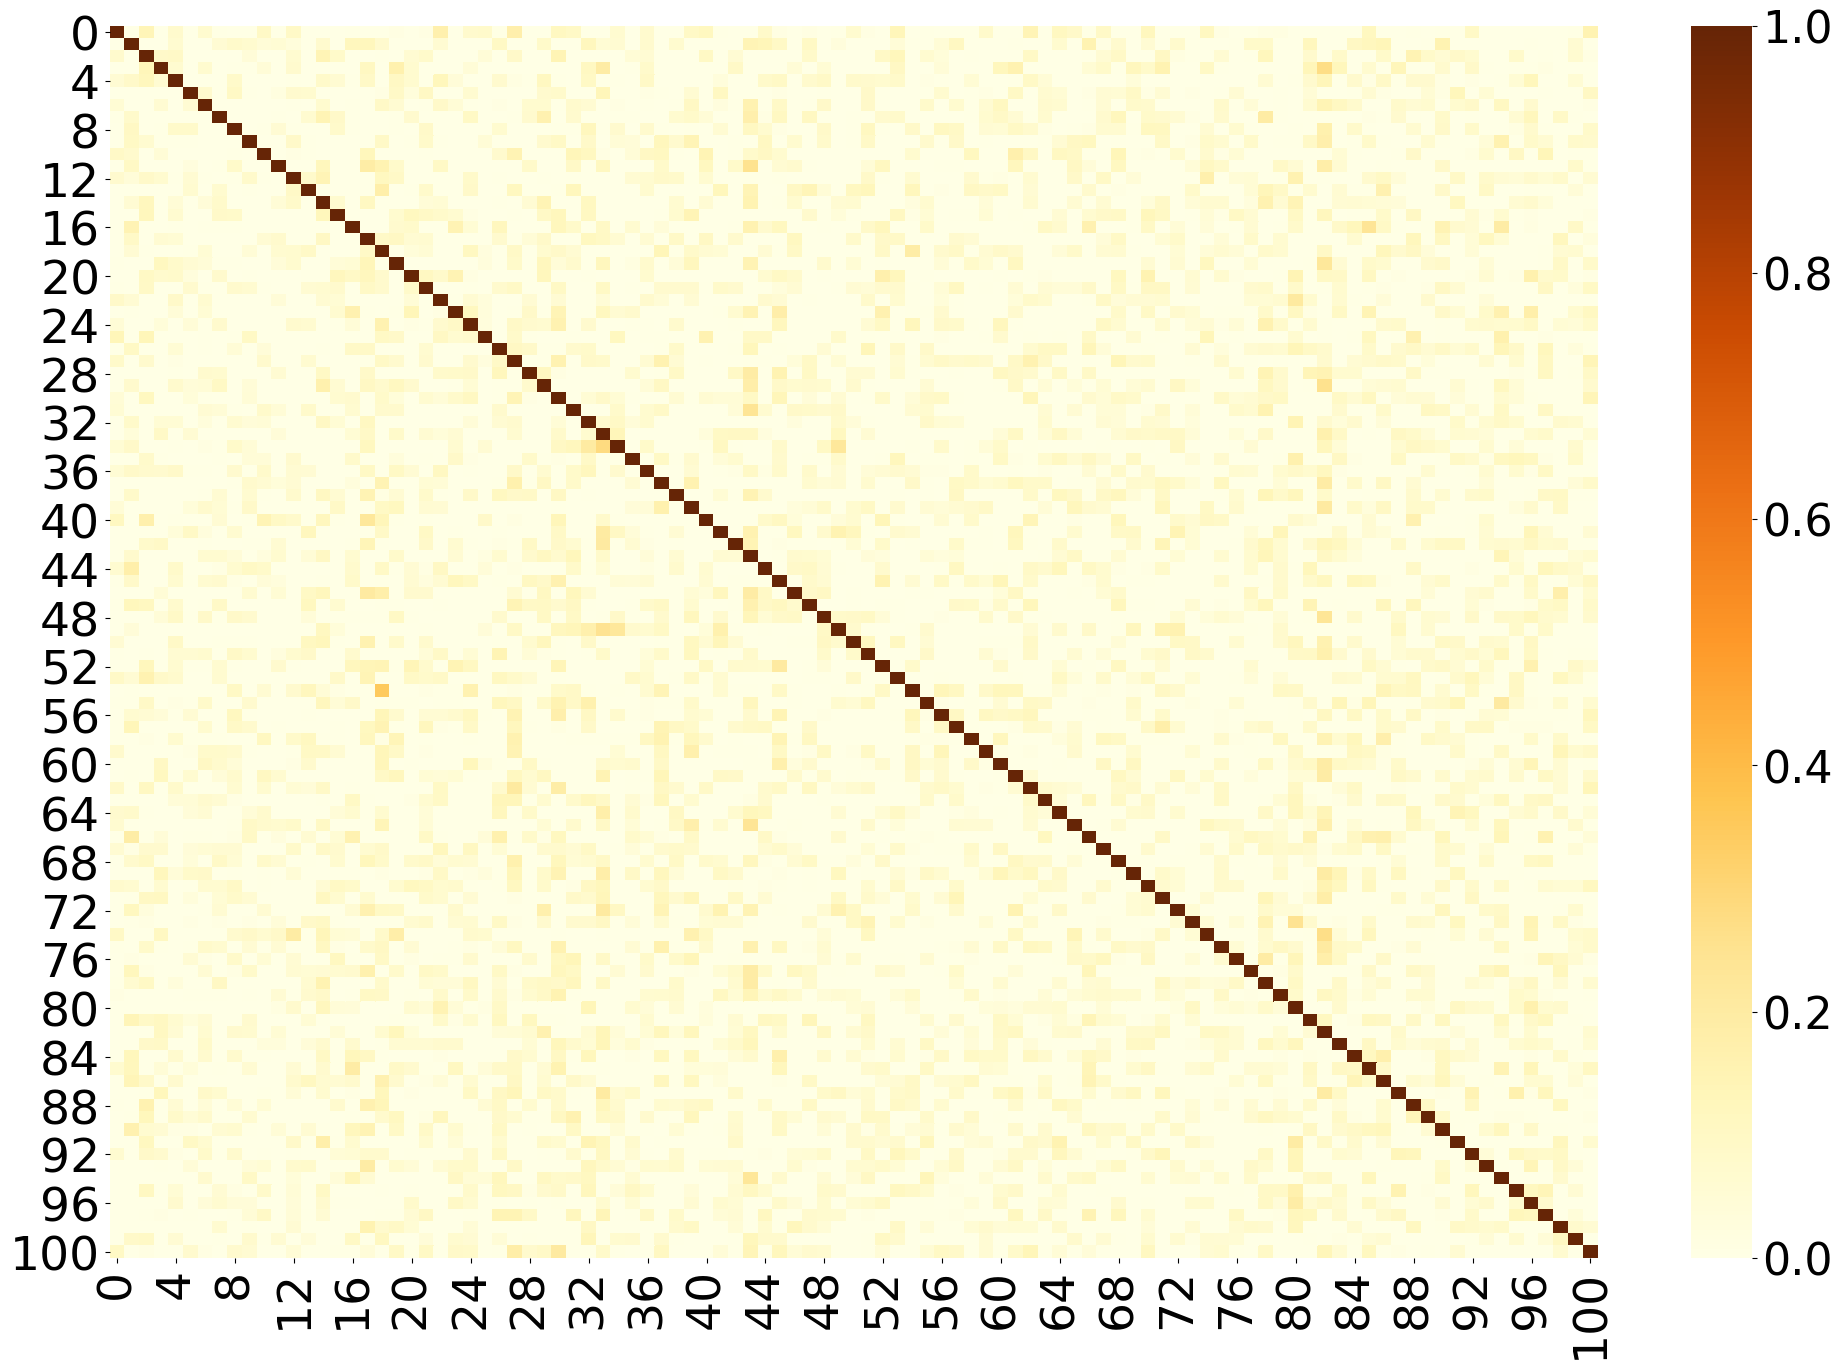
\includegraphics[width=\linewidth /
		2]{figures/experiments/syn/mediamill/MOA_relationship_graph.png}
	\caption[Relación entre etiquetas para cada \textit{stream} generado sobre
		la colección Mediamill.]{Relación entre etiquetas para cada \textit{stream} generado sobre
		la colección Mediamill. Arriba a la izquierda: \textit{Stream} original.
		Arriba a la derecha: \textit{Stream} JC.\@ Abajo a la izquierda:
		\textit{Stream} JC\_BIG.\@ Abajo a la derecha: \textit{Stream} MOA.}
	\label{fig:syn_mediamill_label_relationship}
\end{figure}

También sobre el fenómeno de la dependencia entre etiquetas se pueden hacer
conclusiones similares a las de Enron (ver
figura~\ref{fig:syn_mediamill_label_relationship}). Los gráficos de JC y JC\_BIG
nuevamente reflejan una coloración muy similar al del original, y con una
tonalidad de blanco menos intensa que podría ser producto de un menor valor de
cardinalidad existente en estos \textit{streams} y con respecto al original.

\begin{table}[htbp]
	\centering
	\begin{adjustbox}{max width=\textwidth}
		\begin{tabular}{lllllllll}
	\toprule
	{}            & \multicolumn{2}{l}{mediamill} & \multicolumn{2}{l}{JC} & \multicolumn{2}{l}{JC\_BIG} & \multicolumn{2}{l}{MOA}                                          \\
	\textit{Rank} & Atributo                      & Peso                   & Atributo                    & Peso                    & Atributo & Peso   & Atributo & Peso    \\
	\midrule
	1             & Att46                         & 29202.3                & Att49                       & 28806.8                 & Att49    & 326968 & Att115   & 27933.5 \\
	2             & Att47                         & 28783.2                & Att10                       & 27033.8                 & Att10    & 307780 & Att80    & 23829.8 \\
	3             & Att49                         & 28317.5                & Att57                       & 26862.2                 & Att57    & 305180 & Att64    & 22935.4 \\
	4             & Att109                        & 28158.8                & Att70                       & 26786.1                 & Att70    & 304988 & Att34    & 22479.1 \\
	5             & Att53                         & 28090.6                & Att104                      & 26707.2                 & Att104   & 304122 & Att24    & 22320.1 \\
	6             & Att106                        & 27304.5                & Att26                       & 26393.9                 & Att26    & 300480 & Att89    & 22071.3 \\
	7             & Att51                         & 26977.3                & Att75                       & 26133.6                 & Att75    & 297402 & Att35    & 22061.5 \\
	8             & Att48                         & 26939.2                & Att45                       & 26087.8                 & Att45    & 297152 & Att37    & 22046.7 \\
	9             & Att59                         & 26936.2                & Att108                      & 25858.1                 & Att43    & 294576 & Att98    & 22044.9 \\
	10            & Att107                        & 26546.8                & Att64                       & 25853.8                 & Att64    & 294074 & Att76    & 22041.5 \\
	\bottomrule
\end{tabular}

	\end{adjustbox}
	\caption{Espacio de atributos para \textit{streams} Mediamill.}
	\label{tab:syn_mediamill_features_space}
\end{table}

Finalmente, la figura~\ref{tab:syn_mediamill_features_space} lista los atributos más
frecuentes de cada \textit{stream} y da una idea del espacio de atributos
generado.

\subsection{Clasificaciones}
\label{experimentos_clasificaciones}

La metodología propuesta permitió evaluar los diferentes algoritmos de
clasificación multi-etiqueta para los diferentes \textit{streams} utilizando las
configuraciones sin ensambles, los ensambles de referencias y los métodos de
ensamble propuestos. Los resultados se dividen en métricas de ajustes del modelo
basadas en ejemplos (tabla~\ref{tab:example_based}), métricas basadas en
etiquetas (tabla~\ref{tab:label_based}), y por último las métricas de eficiencia
(tabla~\ref{tab:efficiency}) que cuantifican el tiempo de procesamiento y
espacio de almacenamiento de los modelos. Se marca en negrita la celda
correspondiente al modelo que obtuvo el mejor valor de métrica para la
correspondiente colección de datos. Para cerrar la sección se hace una
comparativa contra experimentos de la literatura de referencia.

\subsubsection{Resultados para Métricas Basadas en Ejemplos}

\begin{table}[htbp]
	\centering
	\begin{adjustbox}{max width=\textwidth}
		\begin{tabular}{l:rrr:rrr:rrr}
	\toprule
	                                            &
	\multicolumn{3}{:c}{\textit{Exact-match}}   &
	\multicolumn{3}{:c}{\textit{Hamming score}} &
	\multicolumn{3}{:c}{\textit{Hamming loss}}                                                                                                     \\
	\textit{Stream}                             & 20ng           & Enron
	                                            & Mediamill      & 20ng           & Enron
	                                            & Mediamill      & 20ng           & Enron          &
	Mediamill                                                                                                                                      \\
	\midrule
	\acrshort{br}                               & 0.228          & 0.018
	                                            & 0.001          & 0.952          & 0.912
	                                            & 0.711          & 0.048
	                                            & \textbf{0.088} & \textbf{0.289}                                                                  \\
	\acrshort{cc}                               & 0.244          & 0.017          & 0.005          & 0.954 & 0.919 & 0.905 & 0.046 & 0.081 & 0.095 \\
	\acrshort{mlht}                             & \textbf{0.315} & \textbf{0.055}
	                                            & \textbf{0.048} & 0.934
	                                            & 0.928          & \textbf{0.957}
	                                            & \textbf{0.066} & 0.072          & 0.043                                                          \\
	\hline
	\acrshort{dwm} (\acrshort{br})              & 0.171          & 0.021
	                                            & 0.001          & \textbf{0.956} & 0.938          & 0.800 & 0.044 & 0.062 & 0.200                 \\
	\acrshort{dwm} (\acrshort{cc})              & 0.167          & 0.024
	                                            & 0.014          & 0.956          & \textbf{0.939} & 0.936 & 0.044 & 0.061 & 0.064                 \\
	\acrshort{ebr}                              & 0.153          & 0.012          & 0.001          & 0.953 & 0.928 & 0.726 & 0.047 & 0.072 & 0.274 \\
	\acrshort{ecc}                              & 0.115          & 0.012          & 0.001          & 0.952 & 0.938 & 0.923 & 0.048 & 0.062 & 0.077 \\
	\hline
	\acrshort{efmp}                             & 0.241          & 0.032          & 0.012          & 0.954 & 0.928 & 0.946 & 0.046 & 0.072 & 0.054 \\
	\acrshort{efmp2}                            & 0.220          & 0.039          & 0.004          & 0.955 & 0.936 & 0.928 & 0.045 & 0.064 & 0.072 \\
	\bottomrule
\end{tabular}

	\end{adjustbox}
	\begin{adjustbox}{max width=\textwidth}
		\begin{tabular}{l:rrr:rrr:rrr:rrr}
	\toprule
	                                        & \multicolumn{3}{:c}{\textit{Accuracy}}     &
	\multicolumn{3}{:c}{\textit{Precision}} &
	\multicolumn{3}{:c}{\textit{Recall}}    & \multicolumn{3}{:c}{\textit{F-score (F1)}}                                                                                                                    \\
	\textit{Stream}                         & 20ng
	                                        & Enron
	                                        & Mediamill                                  & 20ng           & Enron
	                                        & Mediamill                                  & 20ng           & Enron &
	Mediamill                               & 20ng
	                                        & Enron                                      & Mediamill                                                                                                        \\
	\midrule
	\acrshort{br}                           & 0.952
	                                        & 0.912                                      & 0.711          & 0.295
	                                        & 0.326
	                                        & 0.093                                      & \textbf{0.373} &
	\textbf{0.365}                          & \textbf{0.651}
	                                        & \textbf{0.329}                             & 0.345          & 0.163                                                                                           \\
	\acrshort{cc}                           & 0.954                                      & 0.919          & 0.905 & 0.294 & 0.337          & 0.229 & 0.339          & 0.353 & 0.485 & 0.315 & 0.344 & 0.311 \\
	\acrshort{mlht}                         & 0.934
	                                        & 0.928
	                                        & \textbf{0.957}
	                                        & \textbf{0.327}
	                                        & 0.269                                      & \textbf{0.488} &
	0.321                                   & 0.127                                      & 0.378          & 0.324 & 0.172 & \textbf{0.426}                                                                  \\
	\hline
	\acrshort{dwm} (\acrshort{br})          & \textbf{0.956}                             & 0.938          & 0.800 & 0.187 & 0.305          & 0.129 & 0.197          & 0.183 & 0.623 & 0.192 & 0.229 & 0.214 \\
	\acrshort{dwm} (\acrshort{cc})          & 0.956
	                                        & \textbf{0.939}                             & 0.936          & 0.178 & 0.308 & 0.350          & 0.183 & 0.185          & 0.466 & 0.181 & 0.231 & 0.400         \\
	\acrshort{ebr}                          & 0.953                                      & 0.928          & 0.726 & 0.185 & 0.320          & 0.099 & 0.213          & 0.269 & 0.649 & 0.198 & 0.292 & 0.171 \\
	\acrshort{ecc}                          & 0.952                                      & 0.938          & 0.923 & 0.136 & 0.375          & 0.291 & 0.149          & 0.227 & 0.583 & 0.142 & 0.283 & 0.388 \\
	\hline
	\acrshort{efmp}                         & 0.954
	                                        & 0.928                                      & 0.946          &
	0.302                                   & 0.380                                      & 0.404          & 0.361 & 0.351 & 0.418          & 0.328 & \textbf{0.365} & 0.411                                 \\
	\acrshort{efmp2}                        & 0.955
	                                        & 0.936                                      & 0.928          & 0.252 &
	\textbf{0.389}                          & 0.303                                      & 0.277          & 0.303 & 0.516 & 0.264          & 0.340 & 0.382                                                  \\
	\bottomrule
\end{tabular}

	\end{adjustbox}
	\caption{Resultados de métricas basadas en ejemplos sobre los
		\textit{streams} seleccionados para cada algoritmo evaluado.}
	\label{tab:example_based}
\end{table}

\begin{figure}
	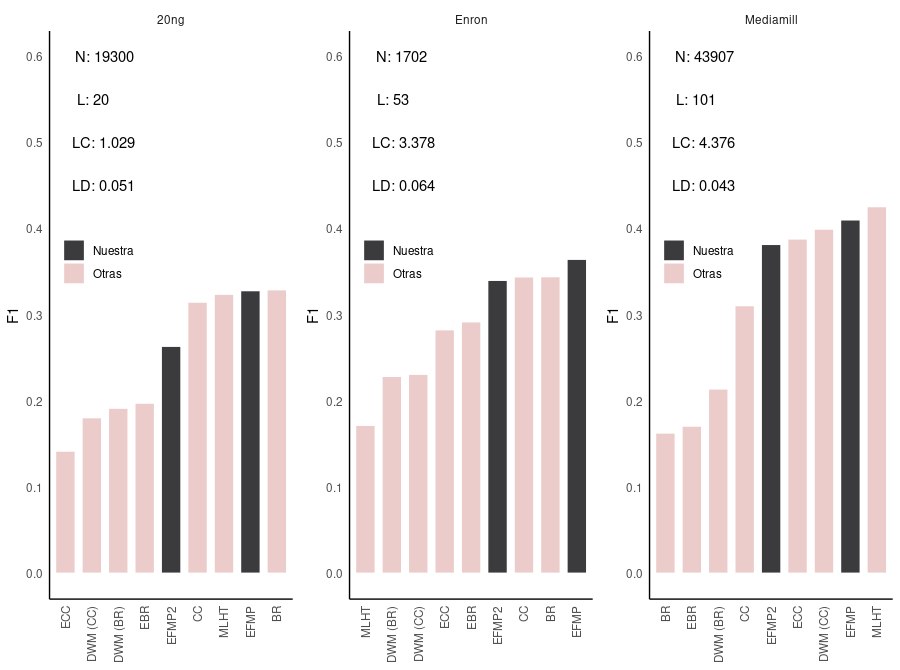
\includegraphics[width=\linewidth,height=10cm]{figures/experiments/classification/f1_ex.png}
	\caption{Comparativa de modelos bajo la métrica \textit{f1} basada en
		ejemplos.}
	\label{fig:comparativa_f1_ex}
\end{figure}

Los valores de F1 obtenidos para la evaluación basada en ejemplos
(Tabla~\ref{tab:example_based}) muestra que \acrshort{efmp} y \acrshort{efmp2}
fueron mejores que los \textit{baselines} de ensambles en todos los casos.
Además, superó a los que no utilizan ensambles en el \textit{stream} de Enron.
En los casos de 20ng, \acrshort{efmp} fue superado en un 0.001\% por
\acrshort{br} y en Mediamill \acrshort{mlht} superó a \acrshort{efmp} en un
0.015\%. Para el caso de \textit{exact-match} el modelo dominante es
\acrshort{mlht}, lo cual es un resultado en consonancia con otros estudios de la
literatura~\cite{read_scalable_2012,osojnik_multi-label_2017,zheng_survey_2020},
y los modelos propuestos se ubican en segundo lugar para dos de las tres
colecciones. En cuanto al \textit{hamming score} los resultados son muy
similares entre colecciones de datos, con los modelos de \acrshort{dwm} sacando
una leve ventaja para 20ng y Enron pero siendo superado por \acrshort{efmp} y
\acrshort{mlht} para Mediamill. También se observan resultados competitivos en
la métrica de \textit{accuracy} donde \acrshort{efmp} supera a todos los modelos
para Enron, incluyendo al de \acrshort{mlht} que es el dominante para Mediamill
y 20ng.

La figura~\ref{fig:comparativa_f1_ex} muestra la comparativa de rendimientos
entre modelos bajo la métrica de \textit{f1}, ordenados desde el menos
performante al más performante y con los modelos aquí presentados en color
negro. Se puede observar cómo en cada \textit{stream} el modelo \acrshort{efmp}
se sitúa entre los dos mejores, siendo el de mejor rendimiento para Enron. De
manera similar, \acrshort{efmp2} se sitúa en cuarto puesto para Enron y quinto
para los demás. Es de notar que otros modelos no logran emparejar rendimientos
entre \textit{streams}, véase el caso de \acrshort{mlht} por ejemplo, que es el
mejor para Mediamill, pero cae en el último puesto para Enron. Este resultado es
coherente con la idea de que los modelos derivados de \acrlong{ht} requieren de
un mayor número de instancias para identificar el mejor punto de corte de un
nodo y lograr mejores evaluaciones~\cite{read_scalable_2012}. Algo similar
sucede con los dos modelos de \acrshort{dwm} que logran valores altos para
Mediamill, pero se ubican entre los tres menos performantes para Enron y 20ng.

\subsubsection{Resultados para Métricas Basadas en Etiquetas}

\begin{table}[htbp]
	\centering
	\begin{adjustbox}{max width=\textwidth}
		\begin{tabular}{lrrrrrrrrr}
	\toprule
	                & \multicolumn{3}{l}{macro\_precision} & \multicolumn{3}{l}{macro\_recall} & \multicolumn{3}{l}{macro\_fscore}                                                         \\
	stream          & 20ng                                 & enron                             & mediamill                         & 20ng  & enron & mediamill & 20ng  & enron & mediamill \\
	\midrule
	br\_nb          & 0.604                                & 0.106                             & 0.062                             & 0.373 & 0.110 & 0.553     & 0.461 & 0.108 & 0.111     \\
	cc\_nb          & 0.667                                & 0.113                             & 0.065                             & 0.340 & 0.097 & 0.150     & 0.450 & 0.105 & 0.091     \\
	dwmc\_br        & 0.781                                & 0.121                             & 0.064                             & 0.196 & 0.031 & 0.418     & 0.314 & 0.049 & 0.111     \\
	dwmc\_cc        & 0.814                                & 0.114                             & 0.068                             & 0.183 & 0.030 & 0.111     & 0.299 & 0.047 & 0.084     \\
	lcht            & 0.546                                & 0.005                             & 0.074                             & 0.318 & 0.016 & 0.030     & 0.402 & 0.008 & 0.043     \\
	me2\_lcht       & 0.699                                & 0.143                             & 0.096                             & 0.276 & 0.059 & 0.173     & 0.396 & 0.083 & 0.124     \\
	me\_lcht        & 0.649                                & 0.114                             & 0.074                             & 0.361 & 0.082 & 0.072     & 0.464 & 0.096 & 0.073     \\
	oza\_ml\_br\_nb & 0.687                                & 0.100                             & 0.062                             & 0.214 & 0.068 & 0.531     & 0.326 & 0.081 & 0.111     \\
	oza\_ml\_cc\_nb & 0.753                                & 0.119                             & 0.049                             & 0.150 & 0.046 & 0.112     & 0.250 & 0.067 & 0.068     \\
	\bottomrule
\end{tabular}

	\end{adjustbox}
	\begin{adjustbox}{max width=\textwidth}
		\begin{tabular}{l:rrr:rrr:rrr}
	\toprule
	                                                &
	\multicolumn{3}{:c}{\textit{Precision} (micro)} &
	\multicolumn{3}{:c}{\textit{Recall} (micro)}    &
	\multicolumn{3}{:c}{\textit{F-score} (micro)}                                                                                                 \\
	\textit{Stream}                                 & 20ng
	                                                & Enron          & Mediamill      & 20ng  &
	Enron                                           & Mediamill      & 20ng           & Enron & Mediamill                                         \\
	\midrule
	\acrshort{br}                                   & 0.552          & 0.330
	                                                & 0.096          &
	\textbf{0.373}                                  & \textbf{0.364} & \textbf{0.673} & 0.445 & 0.347     & 0.168                                 \\
	\acrshort{cc}                                   & 0.597          & 0.364          & 0.224 & 0.340     & 0.353 & 0.485 & 0.433 & 0.358 & 0.306 \\
	\acrshort{mlht}                                 & 0.345          & 0.283
	                                                & \textbf{0.509} & 0.318
	                                                & 0.079          & 0.342          & 0.331
	                                                & 0.124          & \textbf{0.410}                                                             \\
	\hline
	\acrshort{dwm} (\acrshort{br})                  & 0.773          & 0.552          & 0.131 & 0.197     & 0.178 & 0.642 & 0.313 & 0.269 & 0.218 \\
	\acrshort{dwm} (\acrshort{cc})                  & \textbf{0.796} & \textbf{0.569} & 0.328 & 0.183     & 0.179 & 0.463 & 0.298 & 0.272 & 0.384 \\
	\acrshort{ebr}                                  & 0.633          & 0.412          & 0.101 & 0.214     & 0.285 & 0.671 & 0.320 & 0.337 & 0.175 \\
	\acrshort{ecc}                                  & 0.644          & 0.534          & 0.299 & 0.150     & 0.242 & 0.579 & 0.243 & 0.333 & 0.395 \\
	\hline
	\acrshort{efmp}                                 & 0.586          & 0.417
	                                                & 0.384          & 0.361          & 0.339
	                                                & 0.403          &
	\textbf{0.447}                                  & \textbf{0.374} & 0.393                                                                      \\
	\acrshort{efmp2}                                & 0.644          & 0.498          & 0.305 & 0.276     & 0.293 & 0.511 & 0.387 & 0.369 & 0.382 \\
	\bottomrule
\end{tabular}

	\end{adjustbox}
	\caption{Resultados de métricas basadas en etiquetas sobre los
		\textit{streams} seleccionados para cada algoritmo evaluado.}
	\label{tab:label_based}
\end{table}

\begin{figure}
	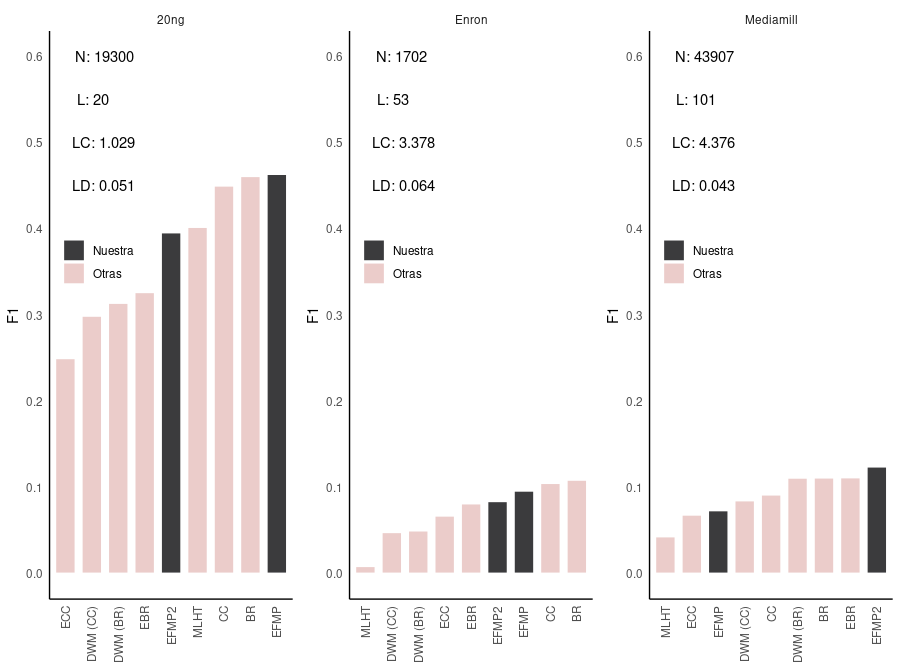
\includegraphics[width=\linewidth,height=10cm]{figures/experiments/classification/f1_macro.png}
	\caption{Comparativa de modelos bajo la métrica \textit{f1} con promedio
		macro, basada en etiquetas.}
	\label{fig:comparativa_f1_macro}
\end{figure}

\begin{figure}
	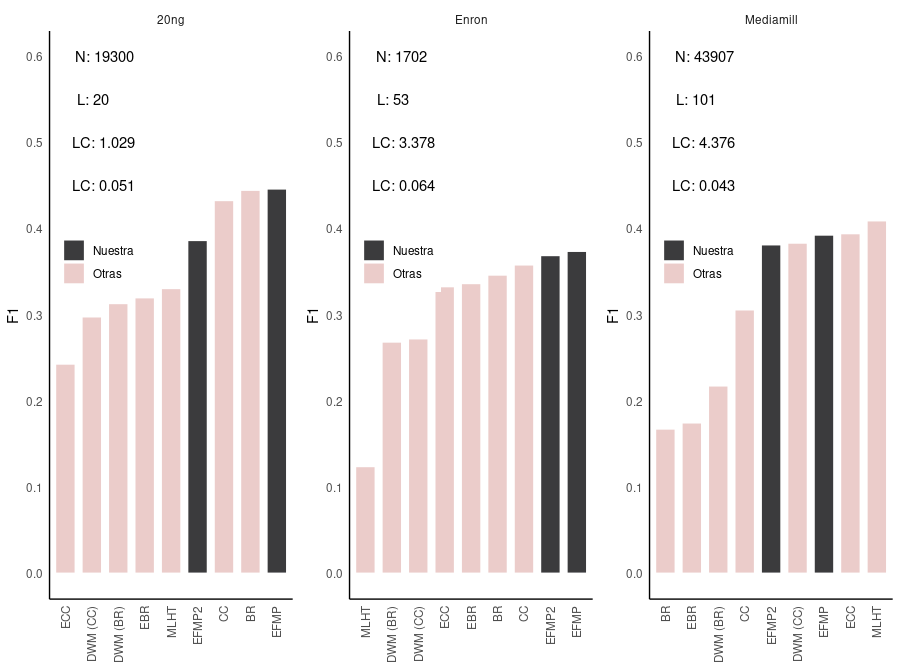
\includegraphics[width=\linewidth,height=10cm]{figures/experiments/classification/f1_micro.png}
	\caption{Comparativa de modelos bajo la métrica \textit{f1} con promedio
		micro, basada en etiquetas.}
	\label{fig:comparativa_f1_micro}
\end{figure}

La métrica de \textit{f1} macro muestra resultados favorecedores para los
modelos presentados. \acrshort{efmp2} obtuvo un valor superior para Mediamill y
\acrshort{efmp} fue el mejor para 20ng y el segundo mejor para Enron, por
centésimas de diferencia con respecto al modelo \acrshort{br}. En lo que
respecta a la comparativa entre soluciones de ensambles, \acrshort{efmp} y
\acrshort{efmp2} superan a las demás para todas las colecciones evaluadas.  Con
relación a los modelos de \acrshort{dwm}, estos muestran una disparidad entre
los valores de precisión y \textit{recall}. Véase por ejemplo el caso de
\acrshort{dwm} (\acrshort{cc}) para 20ng, donde logra más de un 0.8 de precisión
(mejor clasificador) pero un \textit{recall} por debajo de 0.2 (segundo peor
clasificador). Mismo caso, pero a la inversa con \acrshort{dwm} (\acrshort{br})
para Mediamill, el cual consigue alrededor de 0.4 de \textit{recall} (tercer
mejor clasificador) pero apenas un 0.06 de precisión (tercer peor
clasificador).  Esta disparidad logra suavizarse en los modelos de
\acrshort{efmp} presentados y se ve reflejado en valores más altos de
\textit{f1}.

También son favorecedores los valores de las métricas de \textit{f1} micro para
los modelos presentados. \acrshort{efmp} es el mejor para las colecciones 20ng y
Enron y es apenas superado por \acrshort{mlht} para el \textit{stream} de
Mediamill. En la comparativa de métodos de ensambles, \acrshort{efmp} es el
mejor modelo para todos las métricas a excepción del caso de \textit{recall}
para Mediamill (donde \acrshort{ebr} obtiene el mejor valor), y los casos de
precisión para Enron y 20ng, donde \acrshort{dwm} (\acrshort{cc}) logra una
clara diferencia. Al respecto de este último modelo se puede hacer las mismas
consideraciones en cuanto a la disparidad entre precisión y \textit{recall}.

Las figuras~\ref{fig:comparativa_f1_macro} y~\ref{fig:comparativa_f1_micro}
muestra la comparativa de rendimientos entre modelos bajo las métricas de
\textit{f1} macro y micro, respectivamente, y con los mejores modelos
posicionados más a la derecha. Para la métrica macro-promediada se puede
observar que al menos uno de los dos modelos de \acrshort{efmp} se posiciona
entre los mejores tres para cada colección y como el mejor método de ensambles.
Lo mismo sucede con la métrica micro-promediada, donde \acrshort{efmp} supera a
los métodos de \acrshort{br} y \acrshort{cc} para 20ng y Enron y queda por
debajo de \acrshort{mlht} y \acrshort{ecc} para Mediamill.

\subsubsection{Resultados para Métricas de Eficiencia}

\begin{table}[htbp]
	\centering
	\begin{adjustbox}{max width=\textwidth}
		\begin{tabular}{l:ccc:ccc}
	\toprule
	                               & \multicolumn{3}{:c}{Tamaño del modelo (kb)} &
	\multicolumn{3}{:c}{Tiempo de ejecución (segundos)}                                                                              \\
	\textit{Stream}                & 20ng                                        & Enron &
	Mediamill                      & 20ng                                        & Enron & Mediamill                                 \\
	\midrule
	\acrshort{br}                  & 31.6
	                               & \textbf{82.9}
	                               & \textbf{18.9}
	                               & \textbf{1:43:26}
	                               & \textbf{0:21:28}
	                               & \textbf{2:08:42}                                                                                \\
	\acrshort{cc}                  & 31.9                                        & 85.1  & 26.7      & 1:45:00  & 0:27:05 & 2:52:36  \\
	\acrshort{mlht}                & \textbf{22.8}                               & 284.7 & 306.0     & 2:22:30  & 0:58:16 & 19:05:49 \\
	\hline
	\acrshort{dwm} (\acrshort{br}) & 305.5
	                               & 782.9                                       & 185.3 & 21:23:37  & 5:15:03  & 1
	día, 4:21:27                                                                                                                     \\
	\acrshort{dwm} (\acrshort{cc}) & 308.4
	                               & 802.7                                       & 262.4 & 21:03:02  & 5:05:56
	                               & 1 día, 12:49:14                                                                                 \\
	\acrshort{ebr}                 & 316.1                                       & 826.8 & 189.2     & 14:14:56 & 3:41:00 & 20:13:01 \\
	\acrshort{ecc}                 & 319.0
	                               & 847.6                                       & 267.2 & 14:35:33  & 4:03:16
	                               & 1 día, 1:23:01                                                                                  \\
	\hline
	\acrshort{efmp}                & 86.4
	                               & 452.8                                       & 351.7 & 5:41:58   & 1:45:51
	                               & 1 día, 0:47:17                                                                                  \\
	\acrshort{efmp2}               & 84.7
	                               & 359.2                                       & 262.2 & 5:36:55   &
	2:03:59                        & 1 día, 6:27:51                                                                                  \\
	\bottomrule
\end{tabular}


	\end{adjustbox}
	\caption{Resultados de métricas de eficiencia sobre los
		\textit{streams} seleccionados para cada algoritmo evaluado.}
	\label{tab:efficiency}
\end{table}

Tal como es de esperar, la tabla~\ref{tab:efficiency} muestra que los modelos
\textit{baselines} que no son soluciones de ensambles hacen un uso de espacio
menor que los modelos de ensambles y logran tiempos de ejecución
significativamente menores. Sin embargo, en la comparativa entre ensambles, los
algoritmos propuestos (\acrshort{efmp} y \acrshort{efmp2}) reducen tanto el
espacio de almacenamiento como el tiempo de procesamiento de los
\textit{streams} de Enron y 20ng. Mientras que para Mediamill, \acrshort{ebr}
hace un uso significativamente menor de tiempo que los ensambles presentados.
Vale destacar que los modelos de \acrshort{efmp} logran mejorar los tiempos de
ejecución de sus predecesores, los ensambles \acrshort{dwm}.

\subsubsection{Comparativa contra Literatura de Referencia}

A partir de los resultados obtenidos se realiza una comparativa contra otros
estudios del campo. A este fin se seleccionaron los trabajos de
\citeauthor{osojnik_multi-label_2017}
(\citeyear{osojnik_multi-label_2017})~\cite{osojnik_multi-label_2017},
\citeauthor{roseberry_multi-label_2018}
(\citeyear{roseberry_multi-label_2018})~\cite{roseberry_multi-label_2018},
\citeauthor{buyukcakir_novel_2018}
(\citeyear{buyukcakir_novel_2018})~\cite{buyukcakir_novel_2018} y
\citeauthor{sousa_multi-label_2018}
(\citeyear{sousa_multi-label_2018})~\cite{sousa_multi-label_2018}. Si bien las
métricas y colecciones utilizadas varían según el estudio, todos los trabajos
parten de una configuración experimental similar a la de este trabajo y usan el
método \textit{prequential} para evaluar rendimientos.

\citeauthor{osojnik_multi-label_2017} presentaron experimentos sobre las
colecciones de 20ng y Enron bajo métricas basadas en ejemplos (\textit{hamming
	score}, \textit{f1} y \textit{exact-match}), métricas basadas en etiquetas
(precisión, \textit{recall} y \textit{f1}, todas ellas con promedio micro y
macro). Comenzando por las métricas basadas en ejemplos, el modelo
\textit{iSOUP-MT} es el que mejor \textit{hamming score} obtiene en sus
estudios, con un valor de 0.9523, y es levemente superado por \acrshort{efmp}
(0.954) y \acrshort{efmp2} (0.955). Para el caso de Enron el ganador es
\textit{iSOUP-MT} (en su versión de ensambles) con un valor de 0.942 y supera a
\acrshort{efmp2} (0.936). En cuanto al \textit{exact-match} nuestras soluciones
superan a la mejor solución de los autores, iSOUP-RT (0.117), en un 2.05\% para
20ng y son superadas en un 6.25\% por el modelo iSOUP-MT para Enron (0.244). En
lo que respecta al \textit{f1}, \acrshort{efmp} supera en un 2.8\% a iSOUP-RT
(0.118) para 20ng y en poco más de un 1\% a iSOUP-MT para Enron (0.329).

Con respecto a las métricas basadas en etiquetas los resultados también
favorecen a los métodos aquí presentados. Para el \textit{stream} 20ng
\acrshort{efmp2} supera en un 25.5\% a iSOUP-RT bajo la métrica de precisión
macro, en un 238\% en \textit{recall} macro a iSOUP-MT y en un 142\% en
\textit{f1} a ese mismo modelo. Para Enron nuestros modelos superan en un 111\%,
156\% y 164\% a iSOUP-RT para las mismas medidas mencionadas, respectivamente.
Las métricas de promedio micro también favorecen a nuestros modelos. Para 20ng
\acrshort{efmp} es superado en un 41.1\% por iSOUP-MT (en versión ensamble) en
precisión, supera en un 213.6\% a iSOUP-MT en \textit{recall} y en un 125\% en
\textit{f1}. Para Enron es superado en 33.3\% por iSOUP-MT (en versión ensamble)
en precisión, pero consigue superar en un 45.5\% a iSOUP-RT en \textit{recall} y
en un 10.8\% en \textit{f1}.

\citeauthor{sousa_multi-label_2018} han presentado experimentos sobre los tres
\textit{streams} y bajo métricas basadas en ejemplos, en particular las de
\textit{accuracy}, \textit{exact-match}, precisión, \textit{recall} y
\textit{f1}. Para la comparativa se toma el mejor modelo de los autores para
cada métrica. Comenzando por la métrica de \textit{exact-match} los autores han
logrado mejores resultados. Nuestros modelos son superados en un 50.6\% para
20ng, en un 71.7\% para Enron y en un 75.5\% para Mediamill. También para la
precisión, recall y \textit{f1} \citeauthor{sousa_multi-label_2018} han logrado
mejores resultados en general.  En precisión logran superar en un 42.5\% a
\acrshort{efmp} para 20ng, en un 25.6\% a \acrshort{efmp2} para Enron y son
superados en un 0.5\% por \acrshort{efmp} para Mediamill. En \textit{recall}
superan en un 27.5\% a nuestros modelos para 20ng, en un 29\% para Enron y en un
7\% para Mediamill.  Finalmente, en \textit{f1} superan en un 37\% a nuestros
modelos para 20ng, en un 23\% para Enron y en un 15\% para Mediamill. No
obstante, los autores no presentan resultados bajo métricas basadas en
etiquetas.

\citeauthor{roseberry_multi-label_2018}, por su parte, diseñaron el modelo
ML-SAM-kNN y lo pusieron a prueba con las tres colecciones y las métricas de
\textit{exact-match} y \textit{f1} basado en ejemplos. En la comparativa
obtuvimos que \acrshort{efmp} es superado en un 26\% para 20ng, en un 86\% para
Enron y en un 92\% para Mediamill. No obstante, bajo la métrica de \textit{f1},
nuestros modelos superan en un 65\% y 229\% a sus modelos para 20ng y Enron
respectivamente y es superado en un 26\% para Mediamill. Los autores no
realizaron pruebas sobre métricas basadas en etiquetas.

Finalmente, \citeauthor{buyukcakir_novel_2018} presentaron el modelo de
ensambles \textit{GOOWE-ML} bajo las métricas de \textit{hamming score},
\textit{accuracy} basado en ejemplos, \textit{f1} basado en ejemplos y
\textit{f1} micro, basado en etiquetas. Si bien realizaron pruebas sobre varios
\textit{streams} el único en común con este trabajo es el de 20ng. Dicho esto,
su modelo consigue mejores valores para las métricas de \textit{f1} micro,
\textit{accuracy}, y \textit{f1} basado en ejemplos (13\%, 24\% y 26\% de
mejora, respectivamente) y peores valores para la métrica de \textit{hamming
	score} donde nuestros modelos lo superan en un 0.3\%.

En resumen, el resultado de los métodos propuestos muestra que son competitivos
respecto a la literatura de referencia. En particular, para las pruebas
realizadas con el conjunto de datos 20NG los valores de \textit{f1} basado en
ejemplos obtenidos superan a~\cite{osojnik_multi-label_2017} pero no son mejores
que otros como~\cite{sousa_multi-label_2018, buyukcakir_novel_2018,
	roseberry_multi-label_2018}.  En las pruebas realizadas con Enron, los métodos
propuestos superan a~\cite{osojnik_multi-label_2017}, duplican el rendimiento
de~\cite{roseberry_multi-label_2018} y son superados
por~\cite{sousa_multi-label_2018}. Finalmente, para el conjunto de datos
Mediamill tanto~\cite{sousa_multi-label_2018}
como~\cite{roseberry_multi-label_2018} superan nuestra propuesta.
